\chapter{From theory and method to visuospatial models and back}

\section{From theory to visuospatial models}

\noindent The following contributions are ways visuospatial models encapsulate theories from my literature review as contributions 1, 2, and 7: Semantic Forms, Query Isomorphs, and TCA Workspace, respectively. \index[terms]{Semantic Forms} 
\index[terms]{Query Isomorphs} \index[terms]{TCA Workspace}

\subsection{Contribution 1. Semantic Forms}
\begin{itemize}
        \item[\textbf{C1}] \textit{Semantic Forms}, a taxonomy of three-dimensional topic model compositions for HITL CATG, HATG, or both.
\end{itemize}

\subsubsection{Vedic entry point to visuospatial epistemology}
A key outcome of my survey of symbols was arriving at two- and three-dimensional representations. Studying the Sri Yantra and the Meru Chakra together catalyzed a significant shift in my work, expanding it from visual to visuospatial epistemology of information visualization and network graphs. This occurred in two steps. 
\index[terms]{Sri Yantra} \index[terms]{Meru Chakra}  \index[terms]{network graph} \index[terms]{visuospatial epistemology}

First, I read the Sri Yantra as a network graph, which extended its significance in my work beyond its more conventional appreciation as a representation of spiritual qualities to the more etymologically encompassing range of the word \textit{yantra} which includes the practical and mechanical attributes of an 'instrument' or 'machine' \citep[p. 28]{buhnemann_mandalas_2003}. The numerous overlapping triangles of the Sri Yantra evoked a sense of movement for me, like moving network graphs of nodes and edges.

Second, I encountered the Meru Chakra in relationship to the Sri Yantra as interdimensional 2D-3D representations of each other. I propose that signify meaning in both their individual complexity and in the way they hold space for meaning across dimensions. This tension across dimensions catalyzed my ongoing fascination with visuospatial epistemology and the various ways we convey meaning using visuospatial signs \citep{anderson_drawing_2018,drucker_graphesis_2014,dubois_systematic_2002,midgley_theory_1998,sevaldson_designing_2022,tversky_barbara_2022}.
\index[terms]{visuospatial epistemology} \index[people]{Drucker, Johanna} \index[people]{Tversky, Barbara} \index[people]{Sevaldson, Birger} \index[people]{Anderson-Tempini, Gemma}
\index[people]{Dubois, Anna} \index[people]{Gadde, Lars-Erik} \index[people]{Midgley, Gerald} 
\index[terms]{visuospatial epistemology}

\subsubsection{Defining Semantic Forms}
My proposal of Semantic Forms in this thesis does not include comprehensive technical specifications for how to algorithmically build them. Instead, I focus on what researchers might do with Semantic Forms if and when they are developed. I make the assumption that it is possible for Semantic Forms to work with vector embeddings and network graphs. I also conjecture that rich TCA graphs can be used to train Language Models by parsing visuospatial forms of knowledge activation.
\index[terms]{Large Language Model (LLM)} 
\index[terms]{Small Language Model (SLM)} 
\index[terms]{Language Model (LM)} 

The sense of visuospatial affords humans a higher bandwidth for information processing than just two-dimensional representation \citep{tversky_barbara_2022}, which could hold a key for managing the complexity of the climate crisis, or at the very least engaging with it with more agency. This section, however, is about the visuospatial models I made and not about their application to climate. 

As an interface, Semantic Forms are dimensionally versatile three-dimensional visuospatial point cloud compositions that can be dimensionally reduced to produce two-dimensional information representations. As a computational tool using Topological Capta Analysis on high-dimensional graphs, dimensional reductions would occur across a much wider range of dimensions. 

In the following section, I describe the geometric fundamentals I derived from surveying two-dimensional information visualization composition; then, as a means of Meta-Systematic Combining (MSC), I added a third dimension. I called the two-dimensional compositions I derive \textit{Semantic Shapes}, and the three-dimensional compositions I derive \textit{Semantic Forms}. I will write geometric shapes and forms in lowercase, like ``circle" and ``sphere"; I will write the shape identifiers names of my Semantic Shapes and Semantic Forms in uppercase, like ``Circle Semantic Shape" and ``Sphere Semantic Form."
\index[terms]{Semantic Forms} \index[terms]{Semantic Shapes}  \index[terms]{Systematic Combining (SC)}


\subsubsection{Topology in Semantic Forms}
Filtration can be used to assess hierarchical structure in weighted networks \citep[p. 11]{giusti_twos_2016}. Therefore, filtration can facilitate Query Isomorph queries across Semantic Forms with a rigorous inspection process of all nodes and edges in a network, allowing the identification and analysis of network isomorphologies across a variety of network formations, nested and hierarchical or not.
\index[terms]{isomorphology} \index[terms]{topology} 

While filtration is necessary for managing higher-dimensional graphs or graphs with a high density of nodes, I offer a complimentary analogy of magnetic form types. These magnetic form types would affect the distribution of nodes and edges in space in distinct arrangements. The Cone Semantic Form, for example, could distribute topic model graph nodes to reveal the divergence or convergence of ideas in a given text. 
\index[terms]{analogy} 
\index[terms]{Cone Semantic Form} 
\index[terms]{morphology}
\index[terms]{isomorphology}

The value of investigating Semantic Shapes and Semantic Forms was supported for me in more contemporary topological literature about network weighting. The torus and the disc are closely related to the forms uniquely suited to manage Global Topological Synchronization (GTS). \footnote{According to Wang et al., two weighted simplicial complexes, the Weighted Triangulated Torus and the Weighted Waffle ``can sustain global synchronization of edge signals” \citep[p. 9]{wang_global_2024}.} We are one step closer to higher-dimensional topic models in which the physical representations of node relationships represent and reveal more complex semantic relationships like syntopical consiliences.
\index[terms]{syntopical consilience} \index[terms]{Semantic Forms} \index[terms]{Semantic Shapes}  \index[terms]{simplicial complex} 
\index[terms]{consilience}

\subsubsection{Magnetic approach to node groups using weighted graphs}
While existing approaches emphasize filtration \citep[p. 11]{giusti_twos_2016}, edge weighting for managing a large number of nodes \citep{kovacs_iterative_2024}, and self-organizing bundling for emphasizing node relationships to increase their visibility \citep[p. 1]{holten_forcedirected_2009}, the literature considered for this thesis did not find any approaches that considered a taxonomical account of the semantic value of geometric forms for their use in the diachronic, topological, and systematic analysis of network graphs of texts.

Building onto the current practices of network graph filtering and labelling nodes using the semantic value of shapes or forms, I propose Semantic Forms as a new approach for revealing semantic relationships in text graphs. One way this would be achieved is by quantifying Peircean modes of reasoning as a means of node clustering. The Semantic Forms, then, would act as ‘magnetic’ fields which influence the placement of nodes and edges in a topic model graph. Depending on the researcher's aims, these semantic forces would act as an organizing principle that influences all graph nodes or a filtered few. Semantic Forms are, in a sense, semantic forces captured as geometric patterns; they are not prescriptive but are meant to be used to arrange nodes in space to reveal characteristics and patterns within a set of topics. By building on the affordances of three- rather than two-dimensional space, emphasizing node arrangement rather than filtering out potentially valuable contextual nodes, Sematic Forms would improve the identification of more relevant nodes and node relationships.
\index[people]{Peirce, Charles Sanders} 

Weighting a network with the characteristics of Peircean induction, deduction, and abduction would imbue network relationships with useful information for clustering nodes in the virtual semantic field using Semantic Forms. For example, Ontological Semantic Network Summaries (OSNS) can be used to determine the semantic (1) impact and (2) ‘direction’ catalyzed by a given term. For example, in the literature of Aristotle, the practice of categorization would (1) be quantified as having a very high impact; (2) its direction would be (2.1) inductive, as a practice for moving from specific observations to general, or syntopically consilient, conclusions, (2.2) deductive, as a prescription for ontological analysis (e.g. the Tree of Porphyry as semantic network of ontology \citep[p. 4-5]{sowa_knowledge_2000}), (2.3) abductive, defined in a Peircean way, as a means of innovating an explanation in compliment to inductive and deductive reasoning \citep[p. 106]{peirce_pragmatism_1960}. For example, in the study of cognition, categorization is both (a) a phenomenon that can be observed as being comprised of specific characteristics and (b) a means of studying a given subject.
\index[people]{Peirce, Charles Sanders} 
\index[people]{Aristotle}
\index[people]{Porphyry}
\index[terms]{Ontological Semantic Network Summaries (OSNS)} \index[terms]{Global Topological Synchronization (GTS)} \index[terms]{abduction}
\index[terms]{Tree of Porphyry}


\subsubsection{Semantic Shapes: two-dimensional geometric network graph}
Parting from the assumption that dots and lines are the necessary representation of one-dimensional linear relationships, or \textit{Semantic Lines}, I developed a list of two-dimensional shapes which summarize node-radiality compositions used in the organization of network graph information visualizations\footnote{Rendgen et al.’s \textit{History of Information Graphics} \citep{rendgen_history_2019} provide a rich source matter for analyzing information visualization composition. Anna Vital’s infographic of infographics \textit{How to think visually using visual analogies} \citep{vital_how_2018} and \textit{The Data Visualisation Catalogue} by Severino Ribecca \citep{ribecca_data_2017} provide categorizations of information visualization compositions types. I found that individual units of information, dots or otherwise, were laid out away from each other in varying radiality configurations with distinct semantic affordances.}, or what I am naming \textit{Semantic Shape}. The rectangle Semantic Shape can be used to illustrate grids, the triangle Semantic Shape can be used to illustrate hierarchical relationships or contingencies, and the Circle Semantic Shape can represent a multidirectional array of triangular Semantic Shapes.
\index[people]{Vital, Anna} \index[people]{Ribecca, Severino} \index[terms]{Semantic Shapes} \index[terms]{Semantic Line} 

\FloatBarrier
The limited number of individual relationships a node can have in a rectangle Semantic Shape benefits applications like algorithmic quantitative analysis in spreadsheets. However, qualitative analysis benefits from the larger range and variable number of nested node relationships possible in the triangle and Circle Semantic Shape. My focus in the following work favours the triangle and Circle Semantic Shape and their role in categorizing compositions for node graph information visualization.
\index[terms]{Semantic Shapes} 

\begin{figure}[h]
    \centering
    \includegraphics[width=0.8\textwidth]{figures/5.1.png}
    \caption[Network graphs as Semantic Shapes]
    {\textbf{Network graphs as Semantic Shapes}. \textit{Left}: Semantic Line one-dimensional network graph line. \textit{Right}: Semantic Shape two-dimensional network graph radiality compositions: the Rectangle, Triangle, and Circle.}
    \label{f5.1}
\end{figure}


\begin{figure}[h]
    \centering
    \includegraphics[width=0.8\textwidth]{figures/5.2.png}
    \caption[Example of circle and triangle Semantic Shape nested in a larger Circle Semantic Shape network graph]
    {\textbf{Example of Circle and Triangle Semantic Shape nested in a larger Circle Semantic Shape network graph.} \textit{Top left}: Obsidian graph view of my research database. \textit{Top right}: Zoomed view of region marked with yellow-green box. \textit{Bottom}: Labelled Semantic Shape on clusters of network nodes.}
    \label{f5.2}
\end{figure}

\FloatBarrier
%Manuel Lima’s categorization of information visualizations circles and trees \citep{lima_book_2014,lima_book_2017} corroborate the value of my proposal for a Circle Semantic Shape and the triangle Semantic Shape as trees. 

\subsubsection{Semantic Forms: three-dimensional composition types in network graphs}
Moving from one-dimensional network graph lines to two-dimensional network graphs, Semantic Shape laid the groundwork for adding a third dimension to my network graph models and a resulting list of \textit{Semantic Forms}. I approached this exercise as both a deconstruction of complex forms and a combination of Semantic Shape. 
\index[terms]{Semantic Shapes} \index[terms]{Semantic Forms} 


\paragraph{Deconstruction of complex forms} \mbox{} \\

Calling back to my preceding work involving visualizations of Vedic principles, namely the chakras, perhaps the most pivotal bridge for me from theological research to this investigation of network graphs was through Vedic spiritual imagery. In particular, two interrelated forms were the object of my delight and fascination: the Sri Yantra and the Meru Chakra. I studied Vedic spirituality under the guidance of Dr. Monisha Bhatia. However, my work in this thesis will emphasize the geometric and visuospatial attributes of the Sri Yantra and the Meru Chakra, rather than understandings of their cosmological attributes.
\index[terms]{Sri Yantra} \index[terms]{Meru Chakra} 
\index[people]{Bhatia, Monisha}

Encountering that a two-dimensional graph of lines like the Sri Yantra could interrelate with a three-dimensional visualization like the Meru Chakra encouraged me to consider the opportunities available in dimensional addition to flat graphs. 
\index[terms]{Sri Yantra} \index[terms]{Meru Chakra} 

By averaging out the different steps, or elevations, of the Meru Chakra, which has “the form of a mountain” \citep[p. 31]{buhnemann_mandalas_2003}, the cone form is evident in its composition. The Sri Yantra itself is composed around a central point and its sets of triangles are outlined by a circle. I arrived at the geometric curiosity of a graph of lines that could be represented as both a circle and a cone, the former being more typical of an information visualization composition and the latter being novel for me as a method for the semantic representation of individual elements in a graph. 
\index[terms]{Sri Yantra} \index[terms]{Meru Chakra} 

Upon considering the shape of the horn torus, its two horn-shaped negative-space dimples are shaped like cones. Motivated by this geometric curiosity, I considered how other simple forms could be understood as parts of the horn torus. Following this line of reasoning, I arrived at the cylinder as the horn torus’s body, which is also the body of a ring torus. Here, I call back to my preamble work, where I illustrated how a series of horn tori form double cones. At this point, it was easy to envision a horn torus without its double-dimple as a network of nodes organized around a central point or a sphere. Through this deconstruction process, in order of arrival, I list here six Semantic Forms: the Horn Torus, the Cone, the Ring Torus, the Cylinder, the Double-Cone, and the Sphere. 
\index[terms]{horn torus} 
\index[terms]{ring torus}
\index[terms]{cylinder}
\index[terms]{cone}
\index[terms]{sphere}
\index[terms]{Horn Torus Semantic Form}
\index[terms]{Ring Torus Semantic Form}
\index[terms]{Cylinder Semantic Form}
\index[terms]{Cone Semantic Form}
\index[terms]{Sphere Semantic Form}


\paragraph{Combination of Semantic Shapes} \mbox{} \\

Through the combination of Semantic Shapes, conversely, to the previously explained process of deconstruction, I arrived at the same six Semantic Forms. I illustrate how in \autoref{f5.3}. I begin with the PKM graphs from Obsidian and Logseq, which are disc-like Circle Semantic Shapes of nodes. I considered a simple dimensional addition to the Circle, which was to add linear extrusion along a perpendicular axis, creating a Cylinder. I added another form of circular complexity to the Cylinder by circling it in on itself into a Ring Torus. Next, I combined the Triangle and the Circle Semantic Shapes to arrive at the Cone and the Double Cone. Next,  I consider the perpendicular placement of two Circle Semantic Shapes intersecting at their centres by which I arrive at the Sphere. Last, I consider that the Ring Torus can be narrowed to shrink its inner radius to a single point, which makes a Horn Torus.
\clearpage
 \index[terms]{Semantic Shapes} \index[terms]{Semantic Forms} 
 
\FloatBarrier
% First Figure
\begin{figure}[p] % Use [p] to place it on a separate page if needed
    \centering
    \includegraphics[width=0.8\textwidth]{figures/5.3.png}
    \caption[Semantic Forms derived from the Circle Semantic Shape and other Semantic Forms]
    {\textbf{Semantic Forms derived from the Circle Semantic Shape and other Semantic Forms.} Systematic Combining was used as dimensional addition to move from two-dimensional to three-dimensional network graph compositions.}
    \label{f5.3}
\end{figure}

% Second Figure
\begin{figure}[p] % Use [p] to place it on a separate page if needed
    \centering
    \includegraphics[width=0.8\textwidth]{figures/5.4.png}
       \caption[Knowledge graph disc and six Semantic Forms]
        {\textbf{Knowledge graph disc and six Semantic Forms}: (a) Circle Semantic Shape knowledge graph, b) Cylinder Semantic Form, (c) Ring Torus Semantic Form, (d) Cone Semantic Form, (e) Double-Cone Semantic Form, (f) Sphere Semantic Form, and (g) Horn Torus Semantic Form. The top row includes more basic forms, and the bottom row includes more geometrically complex ones.}
    \label{f5.4}
\end{figure}
\FloatBarrier

\index[terms]{Ring Torus Semantic Form}
\index[terms]{Horn Torus Semantic Form}
\index[terms]{Cone Semantic Form}
\index[terms]{Double-Cone Semantic Form}
\index[terms]{Sphere Semantic Form}
\index[terms]{Cylinder Semantic Form}



\par
The Semantic Forms are means of three-dimensional topic model node clustering in a semantic field of terms, which reveal relationships like (1) ontological hierarchy of Peircean reasoning modes in which a singular term expresses a general principle and diverse instances of that general principle, (2) cyclicality, and (3) other modes of semantic relationship interpretation in the visuospatial. As a means of capturing hierarchical semantic systems, Semantic Forms have the capacity to nest other Semantic Forms within themselves.
\index[terms]{Semantic Forms}
\index[people]{Peirce, Charles Sanders}

\textbf{The Cone Semantic Form} is perhaps the most direct illustration of this principle because its form physically turns to a single point. \textbf{The Sphere Semantic Form} encompasses a higher number of radii, which accommodates multiple Cones converging to a single point or a series of nested convergence points. \autoref{f6.1},\textit{The Ontological Semantic Network Summary of the Syntopicon’s Great Ideas onto the Tree of Porphyry}, is an example of a dimensionally reduced Cone Semantic Form of consilience-oriented information categorization. \autoref{f6.1} demonstrates that Sowa's sense of philosophical-computational ontology and Adler's interdisciplinary term-indexing \citep{adler_great_1952-2} can be understood as a single system through Aristotelian categorization and Porphyrian semantic network graphing \citep[p. 4-5]{sowa_knowledge_2000}. \textbf{The Cylinder Semantic Form} provides an extruded space of the flat circular graph and traces individual nodes or graphlets across a third axis representing time as a quantified Semantic Line. \textbf{The Ring Torus Semantic Form} accommodates the cone as a structure that feeds back to itself in a cycle. 

The \textbf{Horn Torus Semantic Form} accommodates multiple cycles that exhibit transformation and feeding back into themselves by emerging from a point, changing, and then returning to that same re-origin point. The horn torus has the distinct ability to nest two cone-like structures in its negative space as an opportunity to capture or reveal additional semantic relationships. For instance, a moving Horn Torus Semantic Form network graph, which is used to topic model a text and identify a re-origin point, can also capture the deductive and inductive changes in relationships between ideas in that text or between this given text and other texts by using the horn torus negative-space horn dimples as Cone Semantic Forms. The Cone Semantic Form can be used on its own to model the deductive and inductive reasoning in a text or texts, of course. Static Horn Torus Semantic Form models can benefit from moving components to represent change over time for shifts of reasoning, iterations, building texts onto one another, or changes of popular opinion. Moving horn toroidal models could also be overlaid with each other to compare arguments and isomorphologies of reason.

\index[terms]{Ring Torus Semantic Form} 
\index[terms]{Query Isomorphs}
\index[terms]{Horn Torus Semantic Form} 
\index[terms]{horn torus}
\index[terms]{Cylinder Semantic Form} 
\index[terms]{Semantic Line} 
\index[terms]{Syntopicon} 
\index[terms]{Tree of Porphyry} 
\index[terms]{Ontological Semantic Network Summaries (OSNS)}
\index[people]{Porphyry}
\index[people]{Sowa, John F.}
\index[terms]{consilience}


\paragraph{Moving Semantic Forms} \mbox{} \\
To render the three-dimensional network graphs of these six Semantic Forms, I used Blender to create moving network graph point clouds using Manuel Casasola Merkle’s plexus effect node programming tutorial \citep{casasola_merkle_blender_2022}.
\index[terms]{Blender (software)}

The resulting models captured my idea for a topic modelling interface that uses three-dimensional network graph Semantic Forms with more clarity. The information visualization encoding of Semantic Forms as interface would label categorical and sequential differences between groups of related ideas using nodes colours. Ideas that can be listed across categories would be identified using edges with colours that gradiate between origin the two different node colours. Moving nodes would represent changes in a database over time including occasions when ideas displace or replace other ideas.
\index[terms]{Semantic Forms} \index[terms]{network graph} 

As moving network graph representations of computational text analysis, my Semantic Forms exemplify how Anderson-Tempini's isomorphogenesis \footnote{Isomorphogenesis is described in more detail \autoref{Interdisciplinary visual methods}. As a brief reminder, Anderson-Tempini's term isomorphogenesis refers to the extension of her isomorphology practice used for exploring ``the potentialities of representing morphology as a dynamic and formative process” \citep[p. 179]{anderson_drawing_2018}.} is echoed in Drucker: “We will use the interpretative force of graphical rhetoric as a gesture language of intellectual life, as a way of shaping our communication using the variable dimensions of time and space in ways that print could only hint at, recording as it did the layered, palimpsestic traces of individual and collaborative activities on the enduring substrate of its material surfaces” \citep[p. 197]{drucker_graphesis_2014}. My moving Semantic Form models capture the way in which new information changes the shape of a visuospatial topic model. For a link to view my moving Semantic Forms, see \autoref{Appendix: Thesis website} of the Appendix.
\index[terms]{isomorphogenesis} \index[terms]{Semantic Forms} 
\index[people]{Drucker, Johanna} \index[people]{Anderson-Tempini, Gemma} 




\paragraph{Geometric analysis} \mbox{} \\
I found Semantic Forms are closely related to surfaces of revolution, meaning surfaces ``generated by rotating a two-dimensional curve about an axis” \citep{weisstein_surface_nodate}. Note the similarities to the Semantic Forms in the following examples: ``Examples of surfaces of revolution include the apple surface [similar to the horn torus], cone (excluding the base),[...] cylinder (excluding the ends),[...] lemon surface [similar to the double cone], [...] sphere, [...] and torus” \citep{weisstein_surface_nodate}. At the outset of my research I considered how new forms of spatial network graphs would plot \textit{into} the Semantic Forms, so I considered their surfaces after.
\index[terms]{torus} 
\index[terms]{surfaces of revolution} 
\index[terms]{Semantic Forms} 
\index[terms]{Personal Knowledge Management (PKM)} 
\index[terms]{Ring Torus Semantic Form}
\index[terms]{Sphere Semantic Form}


I anticipate working with Semantic Forms in relation to surfaces of rotation will lead to new methods of network graph plotting. To begin the differentiation of the Semantic Forms’ volume and surface for the next steps of their geometric analysis, I list the Semantic Forms’ volume and surface equations in Cartesian coordinates as a in Appendix \autoref{Semantic Forms equations}.

\index[terms]{torus} 
\index[terms]{surfaces of revolution} 
\index[terms]{Semantic Forms} 
\index[terms]{Personal Knowledge Management (PKM)} 
\index[terms]{Ring Torus Semantic Form}
\index[terms]{Sphere Semantic Form}


\paragraph{Tidiness of the Semantic Form models} \mbox{} \\
While I am observing the geometry of such compositions and providing examples that neatly showcase their shapes and forms, I am not claiming to advocate for node-by-node retrofitting to fit these models, which would be a disservice to the data. Finding patterns in data is difficult in two dimensions, let alone any dimensions above it. In future work, I will investigate mathematical approaches for identifying Semantic Form patterns in large network models of computationally modelled data. The focus of this work is to identify the semantic value of an array of shapes and forms so as to establish which patterns to look for. The finding of these patterns in real data is for another work. \\

By making Semantic Forms, I sought to define the ways geometric form can be given topological versatility in the ways large groups of nodes reveal group semantic relationships, similar to Global Topological Synchronization \citep{bianconi_topology_2024,wang_global_2024}. In the following section, I aim to focus on the smaller network chunks within these more macroscopic murmurations. 
\index[terms]{Semantic Forms} 
\index[terms]{Global Topological Synchronization (GTS)} 
\index[terms]{topology}
\index[people]{Bianconi, Ginestra}
\index[terms]{Semantic Forms}
\clearpage




\section{Contribution 2: Query Isomorphs}
\begin{enumerate}
        \item[\textbf{C2}] \textit{Query Isomorphs} as a means of Topological Capta Analysis (TCA) in HITL CATG using small graph chunks.
\end{enumerate}


\subsection{Defining the Query Isomorph}

I define Query Isomorphs as isomorphic directed graphlets as dimensionally versatile query objects and query interfaces. In this section I explain the meaning embedded in the terms `isomorph' and `query'.


\paragraph{`Isomorph'} \mbox{} \\
The earliest record of the word isomorph I found was by 19th century chemist Eilhard Mitscherlich, as I mention in my introduction, who uses isomorph to describe `sameness of form.' More specifically, Mitscherlich is known for discovering the the law of isomorphism which links a substance's crystal structure to its chemical composition \citetext{\citealp[p. 239]{Berzelius1821Loethrohr}; \citealp{the_editors_of_encyclopaedia_britannica_eilhardt_2024}; \citealp [p. 427-437]{Mitscherlich1820Abhandlungen}; \citealp[p. 239]{Mitscherlich1837Lehrbuch1}}.
\index[terms]{isomorphism}
\index[people]{Mitscherlich, Eilhard}

Borrowing the isomorphism principle from chemistry, I anticipate a link between a text corpus's spatial network graph `crystalizations' and its `datacule' graphlet compositions. I also anticipate that the application of computational chemistry methods like AlphaFold \citep{alphafold_alphafold_2023} will accelerate information science approaches for finding latent isomorphic semantic relationships (problems/solutions, risks/opportunities, etc.) across academic disciplines. The impact of such systems would not only benefit Sustainability Transitions, but all areas of research.
\index[terms]{isomorphism}

Applying computational chemistry to work with isomorphic semantic relationships also has an opportunity to capture semantic change in graphs of three and many more dimensions. Therefore, I also anticipate that the versatility of topology will help working with isomorphic network graphlets across changing position, configuration, and dimension in high-dimensional hypergraphs. 
\index[terms]{isomorphism}

Isomorphism has had a wider range of applications than chemistry evidenced by the interdisciplinary work of Anderson-Tempini \citep{anderson_drawing_2018} across arts and sciences. Further to interpretive scope of this thesis, I align the Query Isomorph thought experiment substantially to Drucker's humanistic design. Drucker asserts that ``\textit{data are capta}, taken not given, constructed as an interpretation of the phenomenal world, not inherent in it" \citep[p. 128]{drucker_graphesis_2014}. The isomorphism of the Query Isomorph reveals what Drucker refers to as the ``constructedness of data as capta" \citep[p. 128]{drucker_graphesis_2014}. For these reasons, I also carry the interpretive interdisciplinarity of Anderson-Tempini's isomorphology in the term Query Isomorph in addition to its chemical origins. 

\index[terms]{morphology}
\index[terms]{isomorphology}
\index[terms]{isomorphism}
\index[terms]{Query Isomorphs}
\index[terms]{capta}


\paragraph{`Query'} \mbox{} \\
Computer scientist John. F. Sowa produced foundational work in the space of using graphs for querying information databases including the development of Query Graphs \citep[p. 313]{sowa_conceptual_1984}. I arrived at the idea of isomorphological query graphlets independently from Sowa, but our work overlaps and merits disambiguation. Query Graphs are related to my Query Isomorphs as mechanisms that help recognize patterns of meaning across different texts. However, Query Isomorphs differ from Query Graphs as \textit{dimensionally versatile} graph elements, which are queryable with TDA and TCA across the modes of KSSTP, and which also function as interface when in the visible three dimensions. The term Query Isomorph carries the term `Query' with respect of the shared lineage of computational graph-based text analysis that includes and has benefited from John F. Sowa's Query Graph development and pedagogy.


\index[terms]{Query Isomorphs} 
\index[terms]{Topological Data Analysis (TDA)}
\index[terms]{Topological Capta Analysis (TCA)}
\index[people]{Sowa, John F.}
\index[terms]{morphology}
\index[terms]{isomorphology}



\subsection{Making a Query Isomorph}

In this section I demonstrate how I designed a Query Isomorph using the literature review of this thesis by setting my semantic scope, and introducing my visualization design.

\subsubsection{Semantic Field \textit{S} and Sample \textit{s}}

To provide an example of the way Query Isomorph term nodes relate to Semantic Forms I set some parameters. Specifically, I set a semantic field, which is ``a set of words which cover a particular semantic domain and bear structured relations with each other" \citep[p. 107]{jurafsky_speech_2024}. 

To arrive at this list, I uploaded my thesis as a PDF to ChatGPT $4$o and parsed its keywords with the following prompt sequence: 

\begin{enumerate}
    \item[\textbf{1}] ``Categorize and list the key words in this document."
    \item[\textbf{2}] ``Write these as a list separated by commas, ranked by their relevance in the text"
\end{enumerate}
    
I imported this list of 756 Comma Separated Values (CSV) to Microsoft Excel.  Next, I reduced the number of terms on this list by removing redundant and less relevant words. I arrived at a list of 310 terms which I called Semantic Field \textit{S}. This list is included in Appendix \autoref{Appendix Semantic Field S}.
\index[terms]{Query Isomorphs}

Sample \textit{s} is a list of nineteen ideas which I arbitrarily selected from Semantic Field \textit{S} for having high importance in my thesis. In \autoref{tab:semantic_fields}, I list the terms from Sample \textit{s} along with the date of their earliest recorded use in my research database and a note of where the idea was first recorded. I use the word `idea' here and not `term' because some terms have changed over time. For example, I first named Query Isomorph `datacule’ as mentioned previously. The idea of isomorphic representations of ideas endures across the change from the term `datacule' to the term `Query Isomorph.' In a sense, this is an example of the textual isomorphogenesis of ideas about the visuospatial isomorphogenesis of ideas.
\index[terms]{Query Isomorphs}



I derived one term in particular as the most summatively descriptive through-line of this thesis: \textit{Computational Semiosis}. I arrived at this term in two steps. First, I drafted the graphs of Query Isomorph \textit{i} that you will encounter in this section, and arrived at the term \textit{Computational Graphesis}. This term encompassed the practice of applying computational methods like TCA to a wide array of ``visual forms of knowledge production" \citep{drucker_graphesis_2014}, what Drucker calls \textit{graphesis}. Seeking to build on Drucker's term by including Tversky's neuroscience of the visuospatial \citep{tversky_barbara_2022}, I returned to Drucker's Greek etymology of \textit{graphesis}. I derived \textit{semiosis} as more fitting for the sensorially decentralizing and diversifying scope of my \textit{visuospatial} forms of Knowledge Production. More specifically, I defined my use of the term semiosis in this thesis as Knowledge Activation across its various modes (KSSTP), and across the interrelated senses used in understanding, including but not limited to the visuospatial. For my updated through-line term, I arrived at the term \textit{Computational Semiosis}, which I included in \autoref{tab:semantic_fields} and the graphs that follow it.

\index[terms]{Query Isomorphs}
\index[terms]{Knowledge Production (KP)}
\index[terms]{Computational Semiosis}





\FloatBarrier
\begin{table}[htbp]
  \centering
  \begin{tabular}{p{0.4cm}p{4cm}p{2.5cm}p{5cm}}
      \toprule
      \textbf{\#} & \textbf{Sample \textit{s} term} & \textbf{Earliest use on record} & \textbf{Note (Place first used in my records and comment)} \\
      \midrule
      1 & Symbol-making & 2022 Jan and earlier & Prior studies: note-taking methods experimentation \\
      2 & Sri Yantra & 2022 Jan and earlier & Prior studies: theology \\
      3 & Network Graphs & 2022 Jan and earlier & Prior studies: note-taking methods \\
      4 & Meru Chakra & 2022 Jan and earlier & Prior studies: theology \\
      5 & Personal Knowledge Management (PKM) & 2022 Jan 12 & Obsidian: first vault \\
      6 & Torus & 2022 Mar 17 & Images: Resonance Science Foundation,  Yin Yang mapped onto Torus (2013) \\
      7 & Graphesis & 2022 May 01 & Images: first reading of Drucker (2014) \\
      8 & Isomorphology & 2022 Jun 21 & Images: first reading of Anderson-Tempini (2018) \\
      9 & Topology & 2022 Nov 22 & Logseq: A. Tindale meeting notes \\
      10 & Spatial Information Visualization Composition (SIVC) & 2022 Nov 30 & Logseq: new term, made during first reading of Saint-Martin (1990) \\
      11 & Semantic Forms & 2023 Jul 31 & Physical notebooks: first sketches of Semantic Forms \\
      12 & Query Isomorphs  & 2023 Aug 06 & Physical notebooks: first sketches of the Query Isomorph, which I then called `datacules' \\
      13 & Topic Models & 2023 Jul 11 & Zotero: InfraNodus software accessed and added \\
      14 & Gigamapping & 2023 Sep 28 & Zotero: Sevaldson (2022) added  \\
      15 & Systematic Combining & 2024 Apr 17 & Zotero: Kjøde (2024) added \\
      16 & Persistence Homology (PH) & 2024 Jun 10 & Zotero: Bianconi (2021) added \\
      17 & Global Topological Synchronization (GTS) & 2024 Jul 15 & Zotero: Wang et al. (2024) added \\
      18 & Computational Semiosis & 2024 Oct 15 & Document Draft: new term, made as thesis through-line \\
      19 & TCA & 2024 Oct 30 & Document Draft: new term, made to apply Drucker's `capta' to TDA \\
      \bottomrule
  \end{tabular}
   \caption[Sample \textit{s} terms chronology]
    {\textbf{Sample \textit{s} terms chronology.}}

  \label{tab:semantic_fields}
\end{table}
\FloatBarrier
\index[terms]{gigamapping}
\index[people]{Anderson-Tempini, Gemma}
\index[people]{Sevaldson, Birger}
\index[people]{Kjøde, Svein Gunnar}
\index[people]{Drucker, Johanna}
\index[people]{Bianconi, Ginestra}
\index[people]{Tindale, Adam}
\index[terms]{morphology}
\index[terms]{isomorphology}
\index[terms]{gigamapping}
\index[terms]{Persistence Homology (PH)}
\index[terms]{Computational Semiosis}
\index[terms]{torus}
\index[terms]{topology}
\index[terms]{Semantic Forms}
\index[terms]{Spatial Information Visualization Composition (SIVC)}
\index[terms]{Topological Data Analysis (TDA)}
\index[terms]{Topological Capta Analysis (TCA)}




\subsubsection{Visualization style for the Query Isomorph}
At this point in the document, I will begin using three-dimensional objects made with Blender. I decided to keep the dark grey background typical of the Blender platform in alignment with Drucker's sense of humanist post-structuralist design, which reveals the ``constructedness of knowledge" \citep[p. 178]{drucker_graphesis_2014} in visuospatial forms of ``knowledge production" \citep{drucker_graphesis_2014}. I used the shape of a Blender icosphere as the form of each node signal spatial interface for Query Isomorphs.
\index[people]{Drucker, Johanna}
\index[terms]{Query Isomorphs}
\index[terms]{Blender (software)}

To design my figures I draw from \textit{Spectrum}, Adobe's design system, and its guide, \textit{Color for data visualization} \citep{adobe_color_2022}. I use its categorical colour palette to represent differences between ideas that operate in different semantic lanes. For example, I use categorical colour distinctions to differentiate between words more closely associated with Semantic Forms, as opposed to the words more closely associated with Query Isomorphs.
 
I use the Adobe \textit{Spectrum} sequential colour palette \citep{adobe_color_2022} to represent ideas that are incrementally different along a semantic spectrum. For example, the gradiating difference between the highly summative$/$less numerous terms like ``Computational Semiosis", and less summative$/$more numerous terms like ``Isomorphology" and ``Topic models".  

I chose the colour of the edges in my moving Semantic Form network graphs to gradiate across the indigo-teal-green continuum in general alignment with the Adobe Spectrum Viridis sequential colour palette. The use of gradient, instead of block hues, represents the subtle semantic gradiation between related ideas that I would use in the topic model of a complex text. 

When iterating my graphs, the more complex illustrations include three sequential colours and three or more categorical colours. In practice, these more complex figures required a lighter colour for the lightest sequential figures. I tested a colour from the same Adobe Spectrum \textit{Color for data visualization} \citep{adobe_color_2022}, specifically the middle colour of its diverging colour palettes, \texttt{\#FFFFE0}(Light yellow). 

In practical application, Light yellow was difficult to distinguish from white annotations, such as axis lines. I tested options for colour options darker than Light yellow colour slightly while keeping it substantially lighter than Light green, and arrived at \texttt{\#FFF7C7} (Lemon chiffon). 

As a result, my figure illustration style guide consisted of four categorical colours and three sequential colours. The categorical colours are: \texttt{\#0FB5AE} (Seafoam 600), \texttt{\#F68511} (Orange 600), \texttt{\#DE3D82} (Magenta 800), \texttt{\#7E84FA} (similar to Indigo 700). For simplicity of description of the illustrations that follow, I will refer to these as the categorical figure colours Teal, Orange, Magenta, and Purple. The sequential figure colours are: \texttt{\#FFF7C7} (Lemon chiffon)), \texttt{\#D2E21B} (Pear), and \texttt{\#7AD151} (Atlantis) to designate high, middle, and low summativeness respectively. I will refer to these as the sequential figure colours: Light yellow, Light green, and Green.
\footnote{Categorical figure colours were not assigned word names by Adobe in \textit{Spectrum} \citep{adobe_color_2022} in addition to their hexcodes, so I included the name provided by the Colblindor Color Name \& Hue tool \citep{fluck_color_2021}.}

I ensured that the colours I chose for my design system adhere to the Adobe Color Blind Safe color checker \citep{adobe_accessibility_2024}. I confirmed that the contrast ratio is higher than the minimum required 3:1 ratio for all colours using WCAG 2.2 Technique G183 \citep{world_wide_web_consortium_w3c_technique_2024}.



\FloatBarrier   
\begin{figure}[h!]
    \centering
    \includegraphics[width=\textwidth]{figures/5 considered.png}
    \caption[Illustration colours considered]
    {\textbf{Illustration colours considered} from the Adobe Spectrum design system \textit{Color for data visualization} \citep{adobe_color_2022}.}
    \label{5 considered}
\end{figure}

\begin{figure}[h!]
    \centering
    \includegraphics[width=\textwidth]{figures/5 selected.png}
    \caption[Illustration colours selected]
    {\textbf{Illustration colours selected} from the Adobe Spectrum design system \textit{Color for data visualization} \citep{adobe_color_2022}.}
    \label{5 selected}
\end{figure}
\FloatBarrier  

\FloatBarrier


\paragraph{Illustrating Sample \textit{s} as network nodes} \mbox{} \\

I applied my visualization style to \autoref{f5.11.Sample s} visualizing each idea as a node paired with a text label. I have arbitrarily designated each node-label pairing as a high-summative node, mid-summative node, or a low-summative node; these three categories were labelled as Light yellow, Light green, or green respectively, as per my selected set of sequential figure colours. On the left, I list all nineteen ideas from Sample \textit{s}, and on the right, I list the nodes I will use in illustrations of Query Isomorph \textit{i}. Neologisms have a tilde beside them (\textasciitilde), and Contributions have an asterisk beside them (*). Note that the names I gave my contributions are also neologisms, so they have both an asterisk (*) and a tilde (\textasciitilde) shown as *\textasciitilde.
\index[terms]{Query Isomorphs}


\begin{figure}[h!]
    \centering
    \includegraphics[width=0.7\textwidth]{figures/5.11.Sample s.png}
    \caption[Sample \textit{s} ideas list and Query Isomorph \textit{i} ideas list]
    {\textbf{Sample \textit{s} ideas list and Query Isomorph \textit{i} ideas list.}}
    \label{f5.11.Sample s}
\end{figure}
\index[terms]{Query Isomorphs}
\FloatBarrier



\paragraph{Timelines of Sample \textit{s} terms} \mbox{} \\
\\
\autoref{f5.11.Time line} illustrates when each idea was first included in my research database on a linear timeline. The purpose of including this timeline is to visualize how much time passed between the inclusion of each idea in Sample \textit{s}. This figure also introduces design components in my Query Isomorph illustrations, which follow later in this section. For example, each node is labelled with a key term in sequential figure hues for high-summative, mid-summative and low-summative term nodes. This illustration also includes the date and origin note from \autoref{tab:semantic_fields}. 
\index[terms]{Query Isomorphs}
\index[terms]{Semantic Forms}


Some Semantic Forms are arranged using rectilinear timelines, like the Cylinder. However, the Ring Torus Semantic Form uses a time \textit{circle} which I designed by transposing \autoref{f5.11.Time line}, the Linear Timeline of terms of Sample \textit{s}, onto the circumference of a circle. 
\index[terms]{torus}
\index[terms]{Semantic Forms}



\FloatBarrier
\begin{figure}[h!]
    \centering
    \includegraphics[width=\textwidth]{figures/5.11.Time line.png}
    \caption[Sample \textit{s} ideas on a rectilinear timeline]
    {\textbf{Sample \textit{s} ideas on a rectilinear timeline.}}
    \label{f5.11.Time line}
\end{figure}

\begin{figure}[h!]
    \centering
    \includegraphics[width=\textwidth]{figures/5.11.Time circle.png}
    \caption[Sample \textit{s} ideas on a timeline transposed onto a circle]{\textbf{Sample \textit{s} ideas on a timeline transposed onto a circle.}}
    \label{f5.11.Time circle}
\end{figure}
\FloatBarrier  


\subsubsection{Query Isomorph \textit{i}: \textit{i} as a name}


The name `i' may seem to point to the popular prefix used to signify individual customizability of many iProducts, but it was named primarily for other reasons. The scholastic practice of incipit identified works by their first few opening words \citep[p. 3]{smith_book_2001} \footnote{For a thorough introduction of the incipit, its medieval use, and its ideological significance, see the introduction of \textit{Book of the Incipit : Beginnings in the Fourteenth Century} \citep[p. 3]{smith_book_2001}.}. First, the `\textit{i}' in Query Isomorph \textit{i}, is an incipit of the word \textit{Isomorph} by using the first letter of its name. Second, as a play on scale using miniature symbolic representation, I use the letter `i' to depict a small person with a body and a head, whimsically calling attention to the ways text and ideas are experienced spatially \citep{tversky_barbara_2022}, like a place that we move through and \textit{with}. Third, and by extension, the `i' is autobiographical in that, like any work, this thesis is in a sense a self-portrait of its maker. \footnote{Federico Fellini stated: “All art is autobiographical; the pearl is the oyster’s autobiography.” \citep[p. 67]{walter_federico_1965}} Fourth, the letter `i' uses one point and one line, the first and first-dimensional building blocks of all network graphs in all dimensions. To articulate this point further in topological terms, because I propose the Query Isomorph as a tool in Topological Capta Analysis, the point of the `i' represents the $0$-dimensional simplex, or the point, and the bar of the `i' represents the $1$-dimensional simplex, or the line segment \citep[p. 3]{maletic_statistical_2011}.
\index[terms]{incipit} \index[terms]{simplex} \index[terms]{network graph} \index[terms]{symbolic representation} \index[terms]{Topological Capta Analysis (TCA)} \index[terms]{Query Isomorphs} 

\clearpage


\subsection{Representing Query Isomorph \textit{i} in two and three dimensions}

 
\begin{figure}[h]
    \centering
    \includegraphics[width=0.8\textwidth]{figures/5.7.Q i.png}
    \caption[Query Isomorph \textit{i} in 2D and 3D]
    {\textbf{Query Isomorph \textit{i} in 2D and 3D.}
}
    \label{f5.7.Q i}
\end{figure}
\index[terms]{TCA Workspace}
\index[people]{Sowa, John F.}
\FloatBarrier


\autoref{f5.7.Q i} is a depiction of how a researcher might query this thesis using Query Isomorph \textit{i} in two-dimensional and three-dimensional directed graphlet formats. \autoref{f5.7.Q i} (a) has eight numbered Query Isomorph graph edges; 1-5 are directed edges which align with the order of ideas in Sample \textit{s}; Note that 4, 5, and 6 indicate that Query Isomorphs lead me to Persistence Homology (PH), which facilitates 5 as a connection from Semantic Forms to Global Topological Synchronization (GTS)- both 4 and 5 are required to move to TCA, which I arrive to through Query Isomorphs first in 6 because I arrive to the topological ideas of PH via Query Isomorphs, and not through Semantic Forms in 7; 8 represents is an example of an undirected Query Isomorph edge in use, meaning the fictional researcher using Query Isomorph \textit{i} in this example is not looking for a particular derivation sequence between these two ideas, Topic Models and TCA in this case. 
\index[terms]{Query Isomorphs}
\index[terms]{Semantic Forms}
\index[terms]{Persistence Homology (PH)}

In \autoref{f5.7.Q i} (a), I depict Query Isomorph \textit{i} in two dimensions. In \autoref{f5.7.Q i} (b), I depict Query Isomorph \textit{i} in three dimensions, which affords a wider range of node placement. Verticality is used as a method to encode hierarchy into the query. For example, by placing a node higher than another, a researcher using this interface would be querying for how TCA acts as a category for Semantic Forms and Query Isomorphs. The depth of the visuospatial input view affords more space for additional cues for hierarchy and sequence through node placement. 
\index[terms]{Query Isomorphs}
\index[terms]{Semantic Forms}

Many people do not read from left to right, so if I were to code this 3D input method, I would make sure to include an option for the TCA Workspace user to adapt their interface to align with a right-left sequential heuristic. For example, a feature that automatically populates directed Query Isomorph edges between nodes depending on their placement along the horizontal axis would adapt to the person’s settings of derivation starting from the left or from the right. To be clear, however, the Query Isomorph edge direction would be customizable and not dependent on the node’s position along a horizontal axis only, as I expect will be required for many different query configurations.

\index[terms]{Query Isomorphs} \index[terms]{Semantic Forms} \index[terms]{Topological Capta Analysis (TCA)} \index[terms]{Global Topological Synchronization (GTS)}
\index[terms]{Semantic Forms}


I conjecture that the benefits of inputting a query of this level of specificity with a directed query graphlet like the Query Isomorph \textit{i} instead of the above natural language query equivalent can save some time. In my experience, queries are often iterated upon to fine-tune desired information and altered when insightful correlations are encountered. It is in this sense that the dimensionally versatile Query Isomorph, as input methods shown in \autoref{f5.7.Q i} (a) and (b), offer value to the TCA Workspace interface by facilitating query iterations through the semiotic affordances of node position and edge direction.
\index[terms]{Query Isomorphs}


\FloatBarrier

\clearpage

\subsubsection{The option to represent Semantic Shapes in three-dimensional space}

\begin{figure}[h!]
    \centering
    \includegraphics[width=\textwidth]{figures/5.9.Semantic Shape Circle.png}
    \caption[Query Isomorph \textit{i} on a Circle Semantic Shape Logseq network graph]
    {\textbf{Query Isomorph \textit{i} on a Circle Semantic Shape Logseq network graph.}}
    \label{f5.9.Semantic Shape Circle}
\end{figure}


\index[terms]{Query Isomorphs}
\index[people]{Sowa, John F.}
\FloatBarrier

\par
I propose that representing the flat Semantic Shapes in three-dimensional space will be valuable. For example, one occasion I expect will be the placement of Query Isomorphs in their 3D input configuration alongside the larger graph from which they are pulled. Since I propose that TCA Workspace can extend the capabilities of PKM platforms, I illustrate here an example of Query Isomorph \textit{i} superimposed onto my Logseq graph. Furthermore, I expect the dimensional versatility of TCA Workspace to include many more applications of models that use both 2D and 3D information visuospatializations. 
\index[terms]{visuospatialization}
\index[terms]{Query Isomorphs}

\newpage

\subsection{Experiments in Visuospatialization: Query Isomorph \textit{i} in six Semantic Forms}
\index[terms]{visuospatialization}
To begin this series of experiments in Computational Semiosis and information visuospatialization, I will illustrate Query Isomorph \textit{i} as it would appear in TCA Workspace if it were coded. By representing Query Isomorph \textit{i} in the following six Semantic Forms, I illustrate the ways the Query Isomorph would be rearranged and warped when placed within the ‘magnetic’ field of each Semantic Form’s semantic force. I made Sample \textit{s} about this thesis to make it easier for the reader to understand how Query Isomorphs and Semantic Forms could be applied to a text by starting from the text we are already discussing. 

\index[terms]{visuospatialization}
\index[terms]{Query Isomorphs}
\index[terms]{Semantic Forms}
\index[terms]{Semantic Forms}

Each of the following illustrations of Query Isomorph \textit{i} in a Semantic Form was rendered by overlaying node-label pairings onto screenshots of my visuospatial Blender Semantic Form models. As a continuation of \autoref{f5.3} and \autoref{f5.4}, I will present my Semantic Forms as pairings. Each coupling includes a simpler Semantic Form followed by one that is more complex. The Semantic Form pairings that follow are Cylinder with Ring Torus, Cone with Double Cone, and Sphere with Horn Torus. 
\index[terms]{Ring Torus Semantic Form}
\index[terms]{Sphere Semantic Form}
\index[terms]{Cylinder Semantic Form}
\index[terms]{Horn Torus Semantic Form}
\index[terms]{Cone Semantic Form}
\index[terms]{Double Cone Semantic Form}
\index[terms]{torus}
\index[terms]{Query Isomorphs}
\index[terms]{Blender (software)}

\clearpage



\subsubsection{Query Isomorph \textit{i} in the Cylinder and Ring Torus Semantic Forms}

\index[terms]{torus}
\index[terms]{Query Isomorphs}





\FloatBarrier
\paragraph{Cylinder Semantic Form} \mbox{} \\

\begin{figure}[h!]
    \centering
    \includegraphics[width=\textwidth]{figures/5.10.Cylinder.png}
    \caption[Cylinder Semantic Form about Query Isomorph \textit{i}]{\textbf{Cylinder Semantic Form about Query Isomorph \textit{i}.} }
    \label{f5.10.Cylinder}
\end{figure}
\index[terms]{Query Isomorphs}
\index[terms]{Cylinder Semantic Form}
\FloatBarrier  

The \autoref{f5.10.Cylinder} Cylinder Semantic Form represents the duration of my research. To assist in placing each idea node accurately along the central axis line that runs through the core of the Cylinder’s barrel, I overlaid the timeline from \autoref{f5.11.Time line} onto the image of the Cylinder Semantic Form. However, also note that nodes closer to the rotational axis line of the cylinder are more general or summative terms. For example, Spatial Information Visualization Composition (SIVC) is a more general idea than Query Isomorphs. Graphs in PKM platforms Obsidian and Logseq tend to place more densely connected terms in the middle of the graph. Since I am representing a series of PKM graphs as the Cylinder Semantic Form, I am adhering to the principle that more densely connected terms, in this case, more general terms, are placed toward the middle of the two-dimensional graph. Conversely, less summative terms, like Persistence Homology (PH), are represented as less densely connected and, as such, placed closer to the periphery of the Cylinder Semantic Form. 
\index[terms]{Spatial Information Visualization Composition (SIVC)}
\index[terms]{Persistence Homology (PH)}

One of the through-lines of my thesis document is Computational Semiosis, which is labelled in \autoref{f5.10.Cylinder} as a light yellow dashed line through the middle of the Cylinder barrel. The metaphor of a ``through-line" can be made visuospatial with TCA as a means to add clarity to a topic model. The through-line acts as a semantic analogue in a Topological Data Analysis Principal Curve, which passes through the ``middle" of a data cloud \citep[p. 1]{kegl_learning_2000}, or mean/average line. 

To ease the reader into the increasingly visually dense figures, I have left out Sample \textit{s} term-node pairings in this render of Query Isomorph \textit{i} in \autoref{f5.10.Cylinder}.
\index[terms]{Topological Data Analysis (TDA)}


\FloatBarrier

\paragraph{Ring Torus Semantic Form} \mbox{} \\



\begin{figure}[h!]
    \centering
    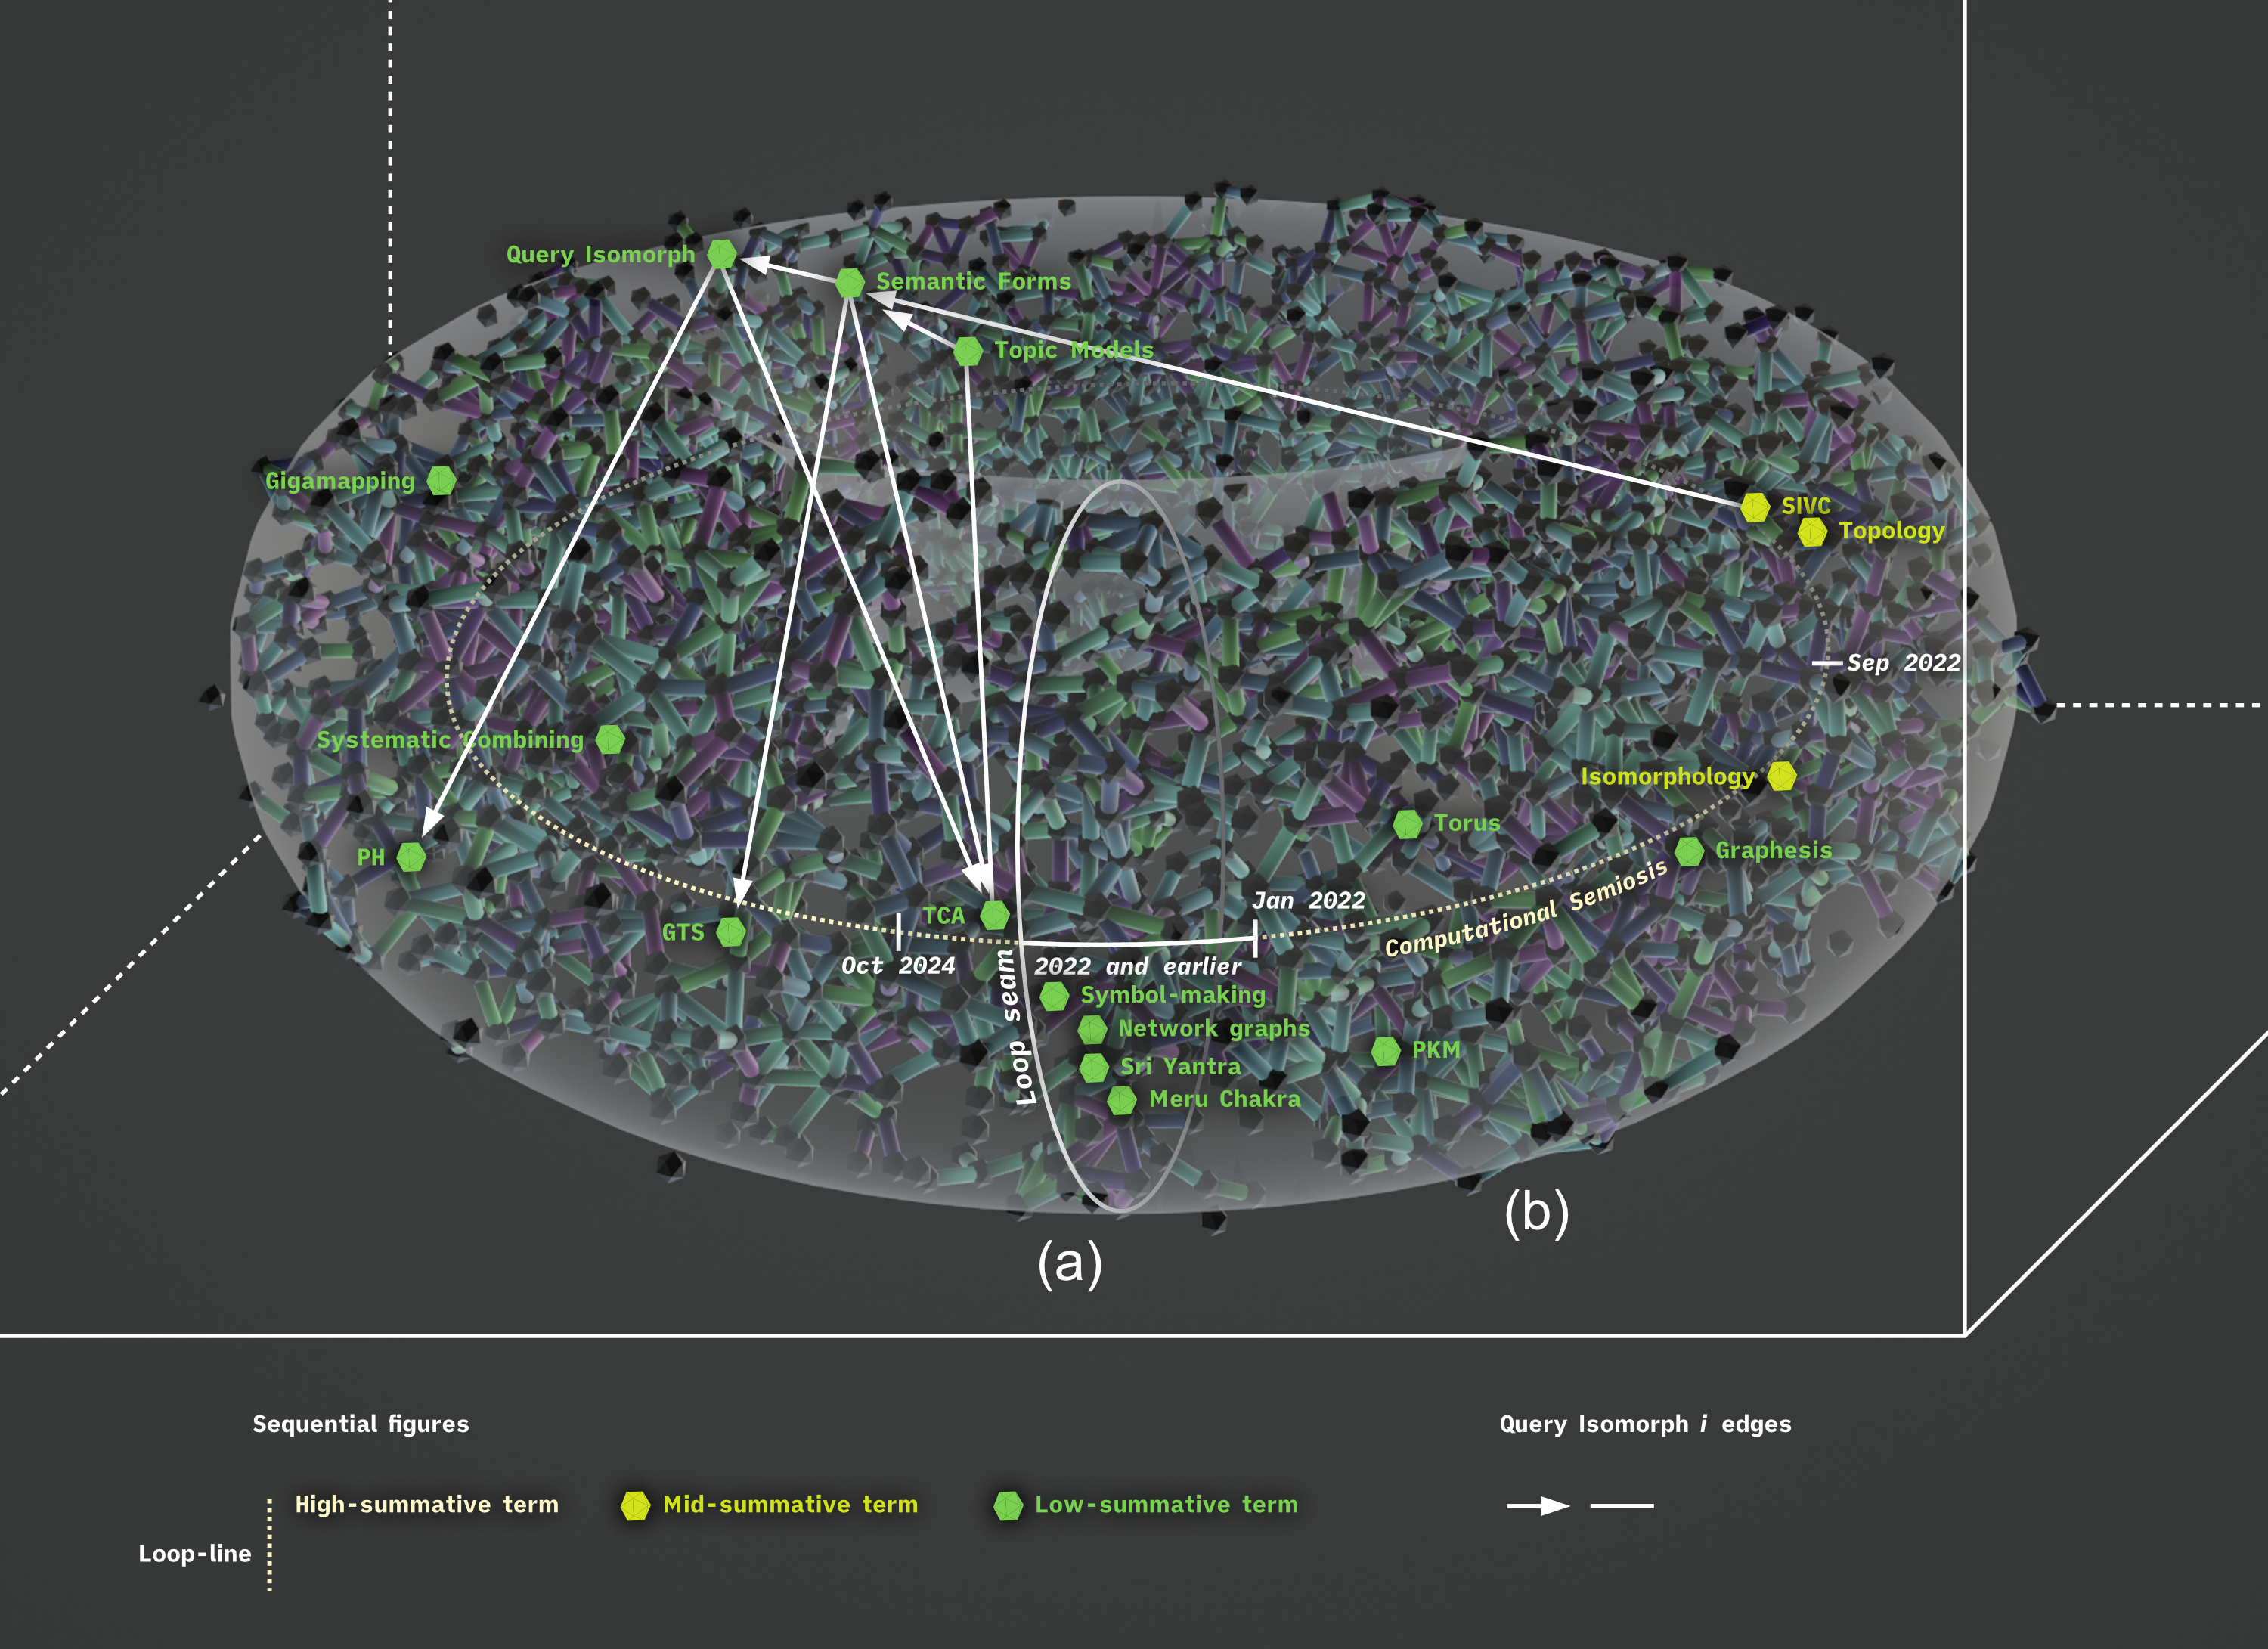
\includegraphics[width=\textwidth]{figures/5.12.RT1.png}
    \caption[Ring Torus Semantic Form about Query Isomorph \textit{i} with rectilinear edges]
    {\textbf{Ring Torus Semantic Form about Query Isomorph \textit{i} with rectilinear edges.} (a) is the Loop seam, and (b) is the Loop-line. Sample \textit{s} terms included for context.}
    \label{f5.12.RT1}
\end{figure}
\index[terms]{Ring Torus Semantic Form}
\FloatBarrier
\index[terms]{torus}

The following figures of Semantic Forms in this series of anticipatory renders of TCA Workspace will contextualize the spatial reconfiguration of Query Isomorph \textit{i} by including term-node pairings of Sample \textit{s}.

I visualized the warp of input Query Isomorph \textit{i} in the output Ring Torus Semantic Form in two ways: In \autoref{f5.12.RT1} I illustrated Query Isomorph edges using rectilinear edges to emphasize the derivation of each Query Isomorph \textit{i} node. In \autoref{f5.12aRT2}, I illustrated the Query Isomorph edges using long arcs that align with the curvature of the Ring Torus. This second style of edges emphasizes the sequence of each Query Isomorph \textit{i} node along the elliptical timeline. I anticipate that toggling between both options will be valuable in the Ring Torus Semantic Form, the Horn Torus Semantic Form, and any future Semantic Forms that involve curved plotting. 
\index[terms]{torus}

\autoref{f5.12.RT1} a) indicates the Loop Seam between the earliest dates and the latest dates along the timeline circle. Dates from Sample \textit{s} that were dated as “2022 and earlier” are labelled in a time segment to the right of the Loop Seam and left of “Jan 2022”. In the case of the Ring Torus Semantic Form, the through-line circles back into itself in what I am calling a Loop-line, indicated in \autoref{f5.12.RT1} b). The Loop-line represents a theme or themes that are both strongly present in a TCA database within a given time range and are expected to be perpetuated if existing semantic patterns continue. 

A computational method to query for topics that act as through-lines about a Query Isomorph in a Ring Torus Semantic Form would accelerate the analysis of texts and text groups. Similar functionality using OpenAI’s GPT-4 to name the relationship between nodes on a graph is already technologically possible, as shown earlier in a discussion about InfraNodus. To apply the Ring Torus Semantic Form, a researcher querying for through-lines using a ring-torus Semantic Form diagram could use this model to identify which topics in a given text most facilitate the continuation of a given thematic cycle.
\index[terms]{torus}


\FloatBarrier
To determine accurate node placement within the Ring Torus Semantic Form, I overlaid \autoref{f5.11.Time circle} as a guide. Specifically, I warped \autoref{f5.11.Time circle} so that its circumference matched the core line running through the Ring Torus in \autoref{f5.12.RT1}. I then moved each node manually along the radii lines of the superimposed and warped \autoref{f5.11.Time circle} either closer to the inner radius or outer radius of the ring torus, depending on my arbitrary measurement of how summative each term is. This technique aligns with the way PKM graphs position nodes by placing more highly connected nodes toward the middle. 
\begin{figure}[h!]
    \centering
    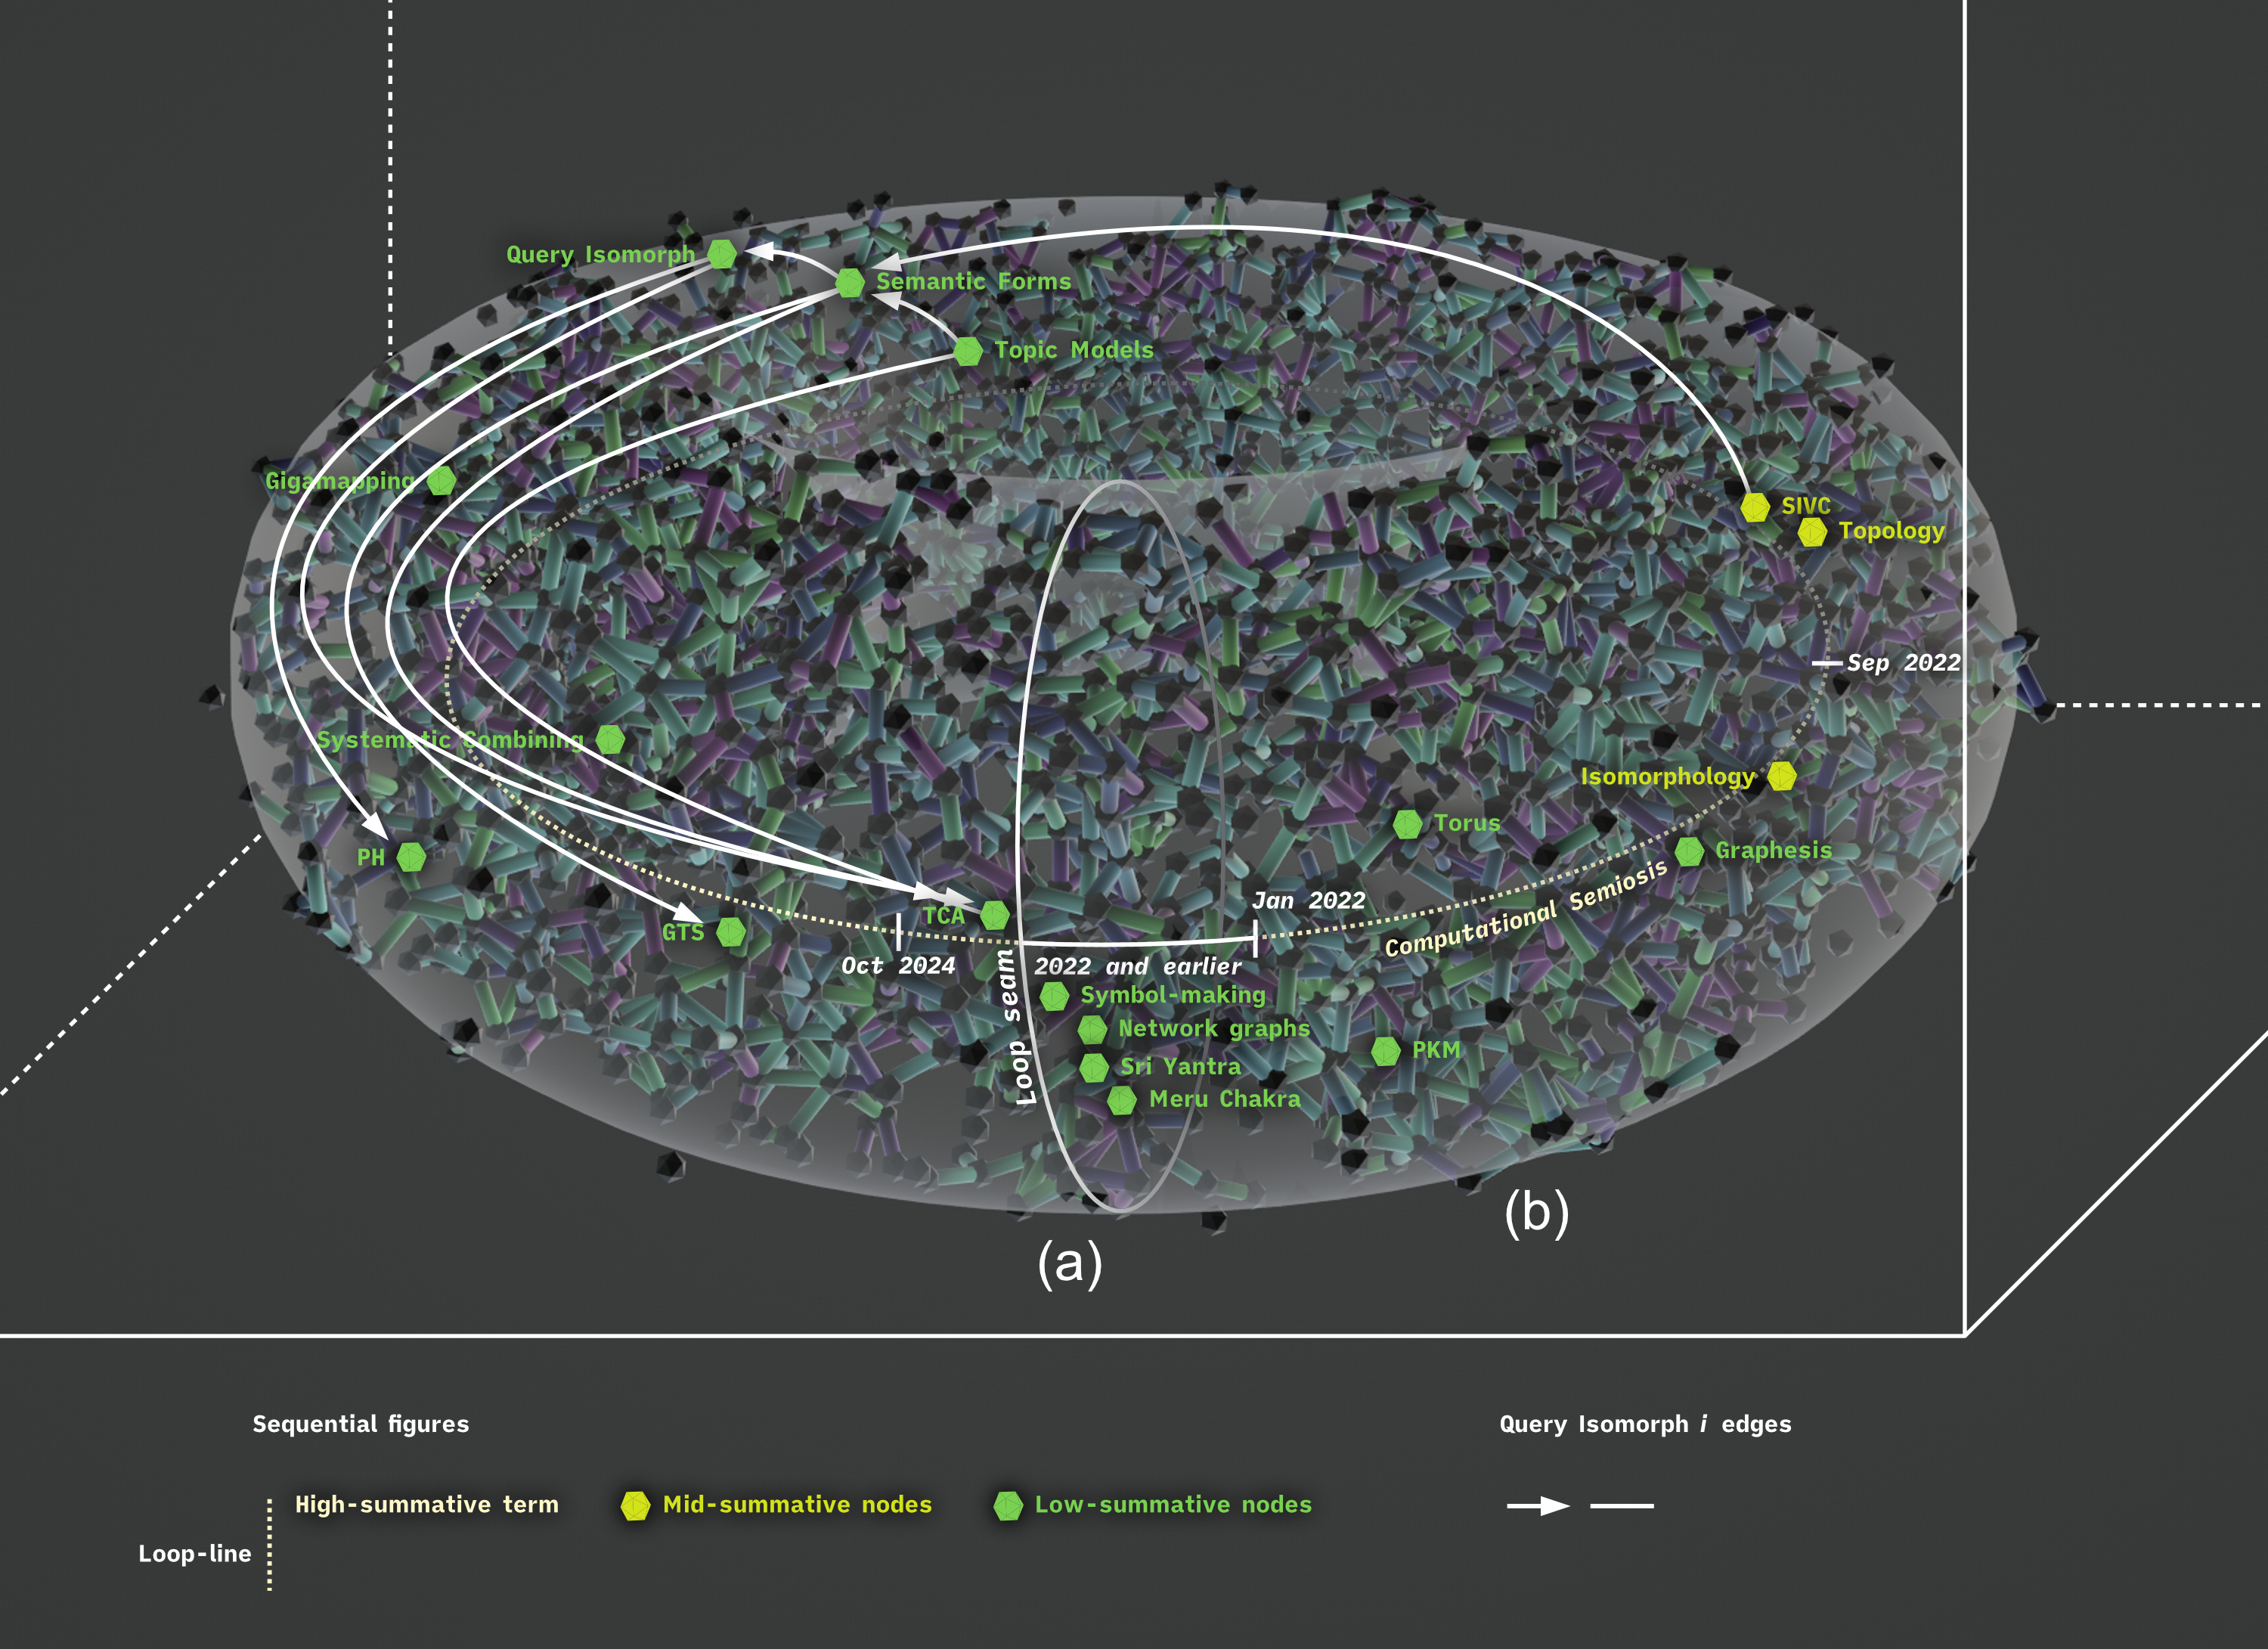
\includegraphics[width=\textwidth]{figures/5.12aRT2.png}
    \caption[Ring Torus Semantic Form about Query Isomorph \textit{i} with arced edges]
    {\textbf{Ring Torus Semantic Form about Query Isomorph \textit{i} with arced edges.} (a) is the Loop seam, and (b) is the Loop-line. Sample \textit{s} terms included for context.}
    \label{f5.12aRT2}
\end{figure}
\index[terms]{Query Isomorphs}
\FloatBarrier  

\clearpage


\subsubsection{Query Isomorph \textit{i} in the Cone and Double Cone Semantic Forms}

\paragraph{Cone Semantic Form} \mbox{} \\

\begin{figure}[h!]
    \centering
    \includegraphics[width=\textwidth]{figures/5.13.Cone.png}
    \caption[Cone Semantic Form about Query Isomorph \textit{i}]
    {\textbf{Cone Semantic Form about Query Isomorph \textit{i}. }Sample \textit{s} terms included for context.}
    \label{f5.13}
\end{figure}
\FloatBarrier  


As opposed to chronological sequence captured in the Cylinder and Ring Torus Semantic Forms, I doubly encode node summativeness in the Cone Semantic Form  using colour and placement. Highly summative nodes are hued light yellow or yellow and placed closer to the Cone's peak, while mid-summative or low-summative nodes are hued green and placed in the middle of the cone or toward its base. Query Isomorph \textit{i} is labelled by connecting its nodes with white edges. 

%Applies to the Ontological Semantic Network Summaries in that the terms which are fewer in number towards the top point are the most summative and have the most subsequent terms derived from them.

\index[terms]{Query Isomorphs}
\index[terms]{torus}
\index[terms]{Semantic Forms}
\index[terms]{Ontological Semantic Network Summaries (OSNS)}
\FloatBarrier


\clearpage

\paragraph{Double Cone Semantic Form} \mbox{} \\


\begin{figure}[h!]
    \centering
    \includegraphics[width=\textwidth]{figures/5.14.DoubleCone.png}
    \caption[Double Cone Semantic Form about Query Isomorph \textit{i}]{\textbf{Double Cone Semantic Form about Query Isomorph \textit{i}.} Sample \textit{s} terms included for context.}
    \label{f5.14.DoubleCone}
\end{figure}
\index[terms]{Query Isomorphs}
\FloatBarrier  

Using the Double Cone Semantic Form, I represent deduction and induction using node divergence and convergence, respectively. Building off the node group label style of InfraNodus \citep{paranyushkin_infranodus_nodate-2}, I hue Theology terms in purple, Semiosis terms in Orange, and 3D information visualization composition terms in Teal, and Graph Math terms in Magenta. My design of the Double Cone Semantic Form follows important precedents; as traced by Sevaldson \citep[p. 102]{sevaldson_designing_2022}, these include Pappus (290-350) \citep[p. 7]{hinitikka_method_1974}, Bánáthy’s model \textit{The dynamics of divergence and convergence} \citep[p. 75]{banathy_designing_1996}, and the British Design Council's Double Diamond framework \citep{design_council_history_nodate}. However, my Double Cone Semantic Form methodological proposal differs from these precedents visuospatializing past two dimensions, applicably to HATG and TCA in HITL CATG.


\index[people]{Sevaldson, Birger}
\index[people]{Bánáthy, Béla Heinrich}
\index[people]{Pappus}


\subsubsection{Query Isomorph \textit{i} in the Sphere and Horn Torus Semantic Forms}

\FloatBarrier


\paragraph{Sphere Semantic Form} \mbox{} \\


\begin{figure}[h!]
    \centering
    \includegraphics[width=\textwidth]{figures/5.15.Sphere1.png}
    \caption[Sphere Semantic Form about Query Isomorph \textit{i}]
    {\textbf{Sphere Semantic Form about Query Isomorph \textit{i}.} This Sphere Semantic Form contains three Cone Semantic Forms: (a) which is about Spatial Information Visualization Composition and Isomorphology, (b) which is about text graph methods of visuospatial knowledge production, and (c) which is about Topology. Sample \textit{s} terms included for context.}
    \label{5.15.Sphere1}
\end{figure}
\index[terms]{Query Isomorphs}
\FloatBarrier  

The Sphere Semantic Form is similar to the Cone Semantic Form in that it represents hierarchical relationships between nodes. However, while the Cone Semantic Form can represent various hierarchies within itself, it predominantly represents one hierarchy. The Sphere Semantic Form effectively represents multiple cone semantic forms, increasing the number of hierarchies that can be represented. 
\index[terms]{Semantic Forms}

\autoref{5.15.Sphere1} illustrates how the high-summative node Computational Semiosis is shared by three Cone Semantic Forms: (a) which is about Spatial Information Visualization Composition and Isomorphology, (b) which is about text graph methods of visuospatial knowledge production, and (c) which is about Topology.  
\index[terms]{topology}
\index[terms]{Semantic Forms}
\index[terms]{Spatial Information Visualization Composition (SIVC)}
\index[terms]{isomorphology}

I present the Sphere Semantic Form with nested Cone Semantic Forms to illustrate an additional notation method for grouping nodes that does not depend on colour encoding like in \autoref{f5.14.DoubleCone}, which increases the researcher's ease of interpretation and avoids opportunities for accessibility issues related to colour blindness. In the same way that the Circle Semantic Shape can contain and overlap with Triangle and Circle Semantic Shapes, like in the Obsidian knowledge graph in \autoref{f5.2}, the Sphere Semantic Form can nest and overlap with Cone and Sphere Semantic Forms. The number of nodes that can be organized in nested hierarchies of Semantic Forms is substantially more than the nodes that can be represented in a Circle Semantic Shape due to their dimensional difference. I expect that testing user experience of reading node hierarchies in Semantic Forms versus Semantic Shapes will reveal results consistent with Ware and Mitchell's \textit{Visualizing graphs in three dimensions} \citep[p. 10]{ware_visualizing_2008} in which users will be able to benefit significantly from a three-dimensional interface for dense graphs.
\index[terms]{Semantic Forms}
\clearpage

\FloatBarrier


\paragraph{Horn Torus Semantic Form} \mbox{} \\

\begin{figure}[h!]
    \centering
    \includegraphics[width=\textwidth]{figures/5.16.HT2.png}
    \caption[Horn Torus Semantic Form about Query Isomorph \textit{i}]
    {\textbf{Horn Torus Semantic Form about Query Isomorph \textit{i}.} Sample \textit{s} terms included for context.}
    \label{f5.16.HT2}
\end{figure}

\index[terms]{Query Isomorphs}
\FloatBarrier  

The Horn Torus Semantic Form is similar to the Ring Torus and Cylinder Semantic Forms in that it represents a series of Circle Semantic Shapes, like a Rolodex \citep{mellby_my_2021} of Obsidian or Logseq graphs in one continuous space as the tube of its body. However, the inner radius of the Ring Torus narrows to a single highly-summative point in the centre of the Horn Torus Semantic Form, making two Cone Semantic Forms which diverge away from each other as negative space outside the Horn Torus. Furthermore, the Loop-line of the Ring Torus Semantic Form is a Zone of Semantic Stasis in the Horn Torus Semantic Form, where ideas are the most consistent and unchanging.

I oriented my model Horn Torus Semantic Form to dimple above and below to evoke trees. The core of the torus represents the trunk which branches up and out, whose leaves fall and transform into the soil, whose nutrients are taken up by the tree's roots–represented by the bottom horn torus dimple. These nutrients are taken back into the tree to the trunk re-origin point in an ongoing cycle of blossoming transformation representative of ideas' flux.
\index[terms]{torus}
\index[terms]{Semantic Forms}

I depict these Horn Torus Semantic Form trajectories of transformation as arcs emerging and returning to their re-origin point. Similarly to the Ring Torus, I used \autoref{f5.11.Time circle} to accurately place term nodes from semantic field \textit{S} with chronological precision onto their respective arcs. The re-origin point, Computational Semiosis, is in the high-summative sequential figure colour light yellow. I depicted the transformation trajectory arcs by labelling them in categorical figure colours: the Semantic Forms arc in Teal, the Query Isomorph arc in Magenta, and the TCA Platform arc in Orange. My transformation trajectory arcs follow the circumference of the torus tube like Rucker's vertical arc orbits representing time in his horn torus model of space-time \citep{rucker_infinity_2005}. However, my transformation trajectory arcs blossom upward and out from the horn torus's centre.
\index[terms]{torus}
\index[terms]{horn torus}
\index[terms]{Semantic Forms}

The Horn Torus Semantic Form differs from the Sphere Semantic Form because it does not nest a variety of Cone Semantic Forms within it at different angles. In fact, the two Cone Semantic Forms at the poles of the Horn Torus Semantic Form represent Gestaltian geometric liminality and interbeing \citetext{\citealp[p. 25]{deleuze_thousand_2007}; \citealp[p. 81-82]{nhat_hanh_world_2008}} of Semantic Form in which the Cone Semantic Form and the Ring Torus Semantic Form are exactly at the brink of being their own forms, being each other, and being a whole that ``is other than the sum of its parts."  \citep[Koffka in Sevaldson, p. 163]{sevaldson_designing_2022}. This thesis is, in many ways, a celebration of the strange and wonderful qualities of the horn torus as a spatial information visualization composition, particularly as a network graph isomorph.
\index[people]{Sevaldson, Birger}
\index[terms]{torus}
\index[terms]{horn torus}
\index[people]{Thích Nhất Hạnh}
\index[people]{Deleuze, Gilles}
\index[people]{Guattari, Félix}
\index[terms]{Semantic Forms}
\index[terms]{Spatial Information Visualization Composition (SIVC)}


\FloatBarrier  
\begin{figure}[h!]
    \centering
    \includegraphics[width=\textwidth]{figures/5.17.HT3.png}
    \caption[Horn Torus Semantic Form about Query Isomorph \textit{i} dimensionally reduced to 2D]
    {\textbf{Horn Torus Semantic Form about Query Isomorph \textit{i} dimensionally reduced to 2D.} Sample \textit{s} terms included for context.}
    \label{f5.17.HT3}
\end{figure}
\FloatBarrier  
\index[terms]{torus}
\index[terms]{Query Isomorphs}




In \autoref{f5.17.HT3} I illustrate two sequences of Horn Torus Semantic Form re-origination in a dimensional \textit{reduction} of \autoref{f5.16.HT2}. On the left, I represent the research before my graduate work at OCAD U in a cycle of divergence and convergence. To the right, I represent my thesis research at OCAD U, which leads to future work. I represent  Query Isomorph \textit{i} by connecting its nodes with white colour edges. The three transformation trajectory arcs from \autoref{f5.16.HT2} are included, but left of the bracket for Thesis research, I added arcs to represent a rough timeline of encountering key formative ideas that preceded my work at OCAD U. First, I added a Theological arc, which includes the terms Theology, Sacred geometry, Vedic meditation, Sri Yantra, and Torus. Note here that the Torus is included earlier in this representation because my fascination with it began with artistic representations of chakras as horn tori. Also, note that the Meru Chakra is placed directly before the beginning of my thesis research arcs and directly before Network graphs. I labelled the Theology arc Purple, the Semantic Forms arc Teal, and the Query Isomorphs arc Magenta because I arrived at a study of network graphs through my fascination with the Meru Chakra. Since the development of Semantic Forms and Query Isomorphs are distinct extensions and disambiguations of a theological principle, I used colour to represent how the Teal Semantic Forms arc and the Magenta Query Isomorphs arc are the separation of blue and red primary colours that make up Purple. Second, the TCA Platform arc extends backward into a short origin story, including Note-taking methods, Mind mapping  \citep{buzan_ultimate_2005}, and Symbol-making. Both arcs and additions left of my Thesis research arcs represent a rough timeline, as I mentioned. I spread each idea along the timeline according to my estimated age when I encountered each idea. The nodes furthest left on the timeline represent the earliest ideas that influenced this research, and the nodes closest to the beginning of my thesis research arcs represent the ideas that were most influential right before beginning my degree at OCAD U. 
\index[terms]{torus}
\index[terms]{Query Isomorphs}
\index[terms]{Semantic Forms}

\clearpage


        

\section{Contribution 7. TCA Workspace, for living webs of thought}
\FloatBarrier  
\begin{enumerate}
      \item[\textbf{C7}] \textit{TCA Workspace}, a methodological prototype of a collaborative HITL CATG + HATG platform to:
    \begin{enumerate}
        \item[(a)] integrate all my thesis contributions (\textit{Semantic Forms}, \textit{Query Isomorphs}, \textit{OSNS}, \textit{Symbol-setting}, \textit{TTG}, and \textit{TCA Researcher Grouping}).
        \item[(b)] facilitate computational interface with Systemic Design methods for visuospatial reasoning encountered through my literature review, such as gigamapping \citetext{\citealp{sevaldson_giga-mapping_2011}; \citealp[p. 26]{sevaldson_designing_2022}} and Systematic Combining \citetext{\citealp[p. 554]{dubois_systematic_2002}; \citealp{kjode_entanglement_2024}}.
    \end{enumerate}
\end{enumerate}
\FloatBarrier  
\index[terms]{Systemic Design}
\index[terms]{gigamapping}
\index[terms]{Systematic Combining (SC)}
\index[terms]{TCA Researcher Grouping}
\index[terms]{Semantic Forms}


TCA Workspace is my proposal for a software platform which will accelerate the computational analysis of texts and graphs with Semantic Forms, Query Isomorphs, Symbol-setting, Ontological Semantic Network Graphs, and Terroir of Text and Graphs (TTG) as independent tools or as combined approaches. The ‘space’ in TCA Workspace invokes the dimensionality of ‘place’ as well as the colliding of electromagnetic particles in nested holarchies of complexity, from the atoms that are our words to the ontologies that are our visible universes. In this sense, TCA Workspace would be a particle accelerator of ideas that activates living webs of thought.
\index[terms]{TCA Workspace}
\index[terms]{Terroir of Text and Graphs (TTG)}
\index[terms]{Symbol-setting}
\index[terms]{Query Isomorphs}




In TCA Workspace, researchers would identify and examine isomorphogenic molecular dynamics simulations of `datacules’, formed of spatial network graphs of entities and relationships in Query Isomorphs and Semantic Forms. Researchers would be able to identify and observe the semantic forces at play in text and graphs, using the rich visuospatial analogues available from across the sciences and humanities, and use computational Topological Capta Analysis. The identification of semantic structures and `datacules' will build on computational chemistry, including the Nobel prize-winning work of David Baker, Damis Hassabis, and John Jumper \citep{jumper_highly_2021,krishna_generalized_2024,the_royal_swedish_academy_of_sciences_press_2024}. Anticipating and developing interdisciplinary methods like the ones proposed in my thesis can be a means of identifying and leveraging latent Sustainability Transitions solutions in the visuospatial meta-patterns of knowledge production.
\index[terms]{TCA Workspace}
\index[terms]{Query Isomorphs}
\index[terms]{Semantic Forms}
\index[terms]{Topological Capta Analysis (TCA)}


In the following sections I invite the consideration of how current approaches to graphs and text are aligned with and can be expanded by the TCA Workspace toolkit.

\subsection{Dimensional addition in Systems Oriented Design with Semantic Forms and Query Isomorphs}
Considering the Meta-Systematic Combining approach I used in this thesis for arriving at Semantic Forms through dimensional addition of Semantic Shape, I propose dimensional addition to Sevaldson’s gigamaps \citep{sevaldson_giga-mapping_2011,sevaldson_designing_2022} as a feature of TCA Workspace that can work concurrently with Semantic Forms and Query Isomorphs. As introduced in \autoref{f5.9.Semantic Shape Circle} with the spatial TCA Workspace representation of the Circle Semantic Shape PKM graph with an overlay of Query Isomorph nodes, I do not intend to represent information in only two-dimensions or three-dimensions in TCA Workspace; instead, I think both can be valuable together in the same render. To illustrate the dimensional versatility of the interface of TCA Workspace, I present two examples of visuospatial gigamaps: \autoref{f5.30.HT gig} my Horn Torus Semantic Form gigamap and \autoref{f5.31.Cone gig} my Cone Semantic Form gigamap.
\index[people]{Sevaldson, Birger}
\index[terms]{Query Isomorphs}
\index[terms]{Systems Oriented Design (SOD)}
\clearpage


\FloatBarrier  
\subsubsection{Gigamaps with Semantic Forms}
\index[terms]{Semantic Forms}


\paragraph{Horn Torus Semantic Form gigamap} \mbox{} \\
\begin{figure}[h!]
    \centering
    \includegraphics[width=0.8\textwidth]{figures/5.30.HT gig.png}
    \caption[Horn Torus Semantic Form gigamap]{\textbf{Horn Torus Semantic Form gigamap.} The spatial network graph in the middle is dimensionally reduced into two-dimensional panes a, b, and c: (a) and (b) reveal the Disintegration and Integration arcs from \autoref{f4.1} which organize the semantic relationships of divergence and convergence from \autoref{f5.16.HT2}. (c) depicts the top view of this Horn Torus Semantic Form as a Mind Map \citep{buzan_ultimate_2005}. Sample \textit{s} terms included for context.}
    \label{f5.30.HT gig}
\end{figure}
\FloatBarrier  
\index[terms]{torus}

In \autoref{f5.30.HT gig}, I depict a conceptual gigamap of a spatial Horn Torus Semantic Form network graph and a sample of dimensional reduction viewing panes. Panes (a) and (c) are depicted as revealing the Disintegration and Integration arcs from \autoref{f4.1} and \autoref{f5.16.HT2}. Pane (b) represents dimensional reduction to a Circle Semantic Shape, in this case as a Mind Map \citep{buzan_ultimate_2005}. The panes' perpendicular angles were chosen for simplicity of introduction, but pane angles would vary widely. Surveying a Semantic Form network graph using multiple angles of dimensionality reduction, algorithmically or not, could reveal significant node correlations that would otherwise be missed. 
\index[terms]{torus}
\clearpage

\FloatBarrier  

\paragraph{Cone Semantic Form gigamap} \mbox{} \\
\begin{figure}[h!]
    \centering
    \includegraphics[width=0.8\textwidth]{figures/5.31.Cone gig.png}
    \caption[Cone Semantic Form gigamap about Query Isomorph \textit{i}]
    {\textbf{Cone Semantic Form gigamap about Query Isomorph \textit{i}.} The network graph is dimensionally reduced in four angles into two-dimensional panes: (a) in a Cone of Plausibility \citep{bezold_overview_1993}, (b) as an inductive and deductive reasoning analysis, (c) as a Horn of Futures model, and (d) as an adaptation of “Diagram of a design process with iterations” \citetext{\citealp[p. 343]{sevaldson_designing_2022}; \citealp{sevaldson_designing_2022-1}}. Sample \textit{s} terms included for context.}
    \label{f5.31.Cone gig}
\end{figure}
\FloatBarrier  

Second, I depict a conceptual gigamap with a Cone Semantic Form network graph dimensionally reduced in four angles: (a) in a Cone of Plausibility \citep{bezold_overview_1993}, (b) as an inductive and deductive reasoning analysis, (c) as a Horn of Futures model, and (d) as an adaptation of “Diagram of a design process with iterations” \citetext{\citealp[p. 343]{sevaldson_designing_2022}; \citealp{sevaldson_designing_2022-1}}, similarly to \autoref{f5.30.HT gig}, these angles are not prescriptive to the practice of Cone Semantic Form gigamapping. 
\index[people]{Bezold, Clement}
\index[people]{Sevaldson, Birger}
\clearpage

\subsubsection{Systematic Combining with Semantic Forms and Query Isomorphs}
Systematic Combining (SC) is a form of Knowledge Production that combines diagrams into larger, more integrated, and capacious models. The driving urgency of my work is Sustainability Transitions, so I examine the doctoral thesis and Systematic Combinations of Svein Gunnar Kjøde, \textit{Entanglement of Systemic Design and Sustainability Transitions} \citep{kjode_entanglement_2024}, as a case study for the existing use of Spatial Information Visualization Composition (SIVC) in Design for Sustainability Transitions. Identifying the current use of SIVC is valuable to me because it demonstrates areas that would benefit from the key functions of TCA Workspace, such as Semantic Forms and Query Isomorphs. 
\index[people]{Kjøde, Svein Gunnar}
\index[terms]{Query Isomorphs}
\index[terms]{Spatial Information Visualization Composition (SIVC)}

I found that Kjøde included or made SIVCs using three geometric forms, which are among my six Semantic Forms, represented in \autoref{f5.23}, \autoref{f5.25},  \autoref{f5.27}. First, the sphere, which organizes the ideas in \autoref{f5.23} the “Floke programme and quadruple helix for stakeholder inclusion” \citep[p. 125]{kjode_entanglement_2024}. Second, the cone, which organizes the ideas in \autoref{f5.25}, Kjøde’s “Relating systemic design practice to socio-technical systems theory and the MLP” \citep[p. 123]{kjode_entanglement_2024}. Third, the cylinder which organizes the ideas in \autoref{f5.27}, Kjøde’s “Praxeological framework for DfST relating to systematic transition initiatives” \citep[p. 144]{kjode_entanglement_2024}. The first two figures have a more self-evident similarity to my Semantic Forms. The third figure, \autoref{f5.27}, is a four-lobed visualization with the words “Systemic Praxeology of DfST” in its centre. This four-lobed figure is indicated to occupy the one-dimensional “Systemic Practice”, which is labelled as a colourful double-directional arrow pointing from the bottom left to the top right. “Systemic Practice” is labelled as one ‘slice’ of a cylindrical spiral labelled with a single-directional arrow and the words “Transition Initiative(s).” To apply my terminology as a summation, Kjøde’s four-lobed “Systemic Praxeology of DfST” is a two-dimensional Circle Semantic Shape in a Cylinder Semantic Form, similar to the composition of \autoref{f5.10.Cylinder} which represents a cylinder of PKM graphs. 
\index[people]{Kjøde, Svein Gunnar}

To relate my work to Kjøde’s, I include a fourth figure, \autoref{f5.28.Kjode b}, which represents how nodes in Sample \textit{s} and Query Isomorph \textit{i} would be positioned in relation to “Systemic Praxeology of DfST” \citep[p. 144]{kjode_entanglement_2024}. This four-lobed form operates similarly to a Circle Semantic Shape, so I place terms with higher summativeness toward the figure’s centre.
\index[people]{Kjøde, Svein Gunnar}
\index[terms]{Query Isomorphs}

\FloatBarrier  
\begin{figure}[h!]
    \centering
    \includegraphics[width=0.5\textwidth]{figures/5.23.png}
    \caption[Spherical SIVC in DfST]
    {\textbf{Spherical SIVC in DfST.} This figure is based on the ``Floke programme and quadruple helix for stakeholder inclusion” in Kjøde \citep[p. 125]{kjode_entanglement_2024}
}
    \label{f5.23}
\end{figure}
\index[people]{Kjøde, Svein Gunnar}

\begin{figure}[h!]
    \centering
    \includegraphics[width=0.5\textwidth]{figures/5.25.png}
    \caption[Conical SIVC in DfST]
    {\textbf{Conical SIVC in DfST.} This figure is based on Kjøde’s ``Relating systemic design practice to socio-technical systems theory and the MLP” \citep[p. 123]{kjode_entanglement_2024}. This figure includes Norwegian terms left of ``Sustainability Transitions” to indicate the ``patchwork of regimes” in overlapping aspects of ``Socio Technical Change”: utbygging, drift, rehabilitering, sanering, and gjenbruk: Utbygging refers to the initial ``development” \citep{cambridge_university_press_utbygging_nodate}; Drift refers to the ongoing operations and management \citep{cambridge_university_press_drift_nodate}; Rehabilitering refers to the ``rehabilitation” or restoration and upgrading of existing structures  \citep{cambridge_university_press_rehabilitering_nodate}; Sanering refers to ``clearing” or sanitation \citep{cambridge_university_press_sanering_nodate-3}; Gjenbruk refers to reusing or recycling \citep{cambridge_university_press_gjenbruk_nodate}.
}
    \label{f5.25}
\end{figure}
\index[people]{Kjøde, Svein Gunnar}




\begin{figure}[h!]
    \centering
    \includegraphics[width=\textwidth]{figures/5.27.png}
    \caption[Cylindrical SIVC in DfST]
    {\textbf{Cylindrical SIVC in DfST.} This figure is based on Kjøde’s ``Praxeological framework for DfST relating to systematic transition initiatives” \citep[p. 144]{kjode_entanglement_2024}.
}
    \label{f5.27}
\end{figure}
\index[people]{Kjøde, Svein Gunnar}



\begin{figure}[h!]
    \centering
    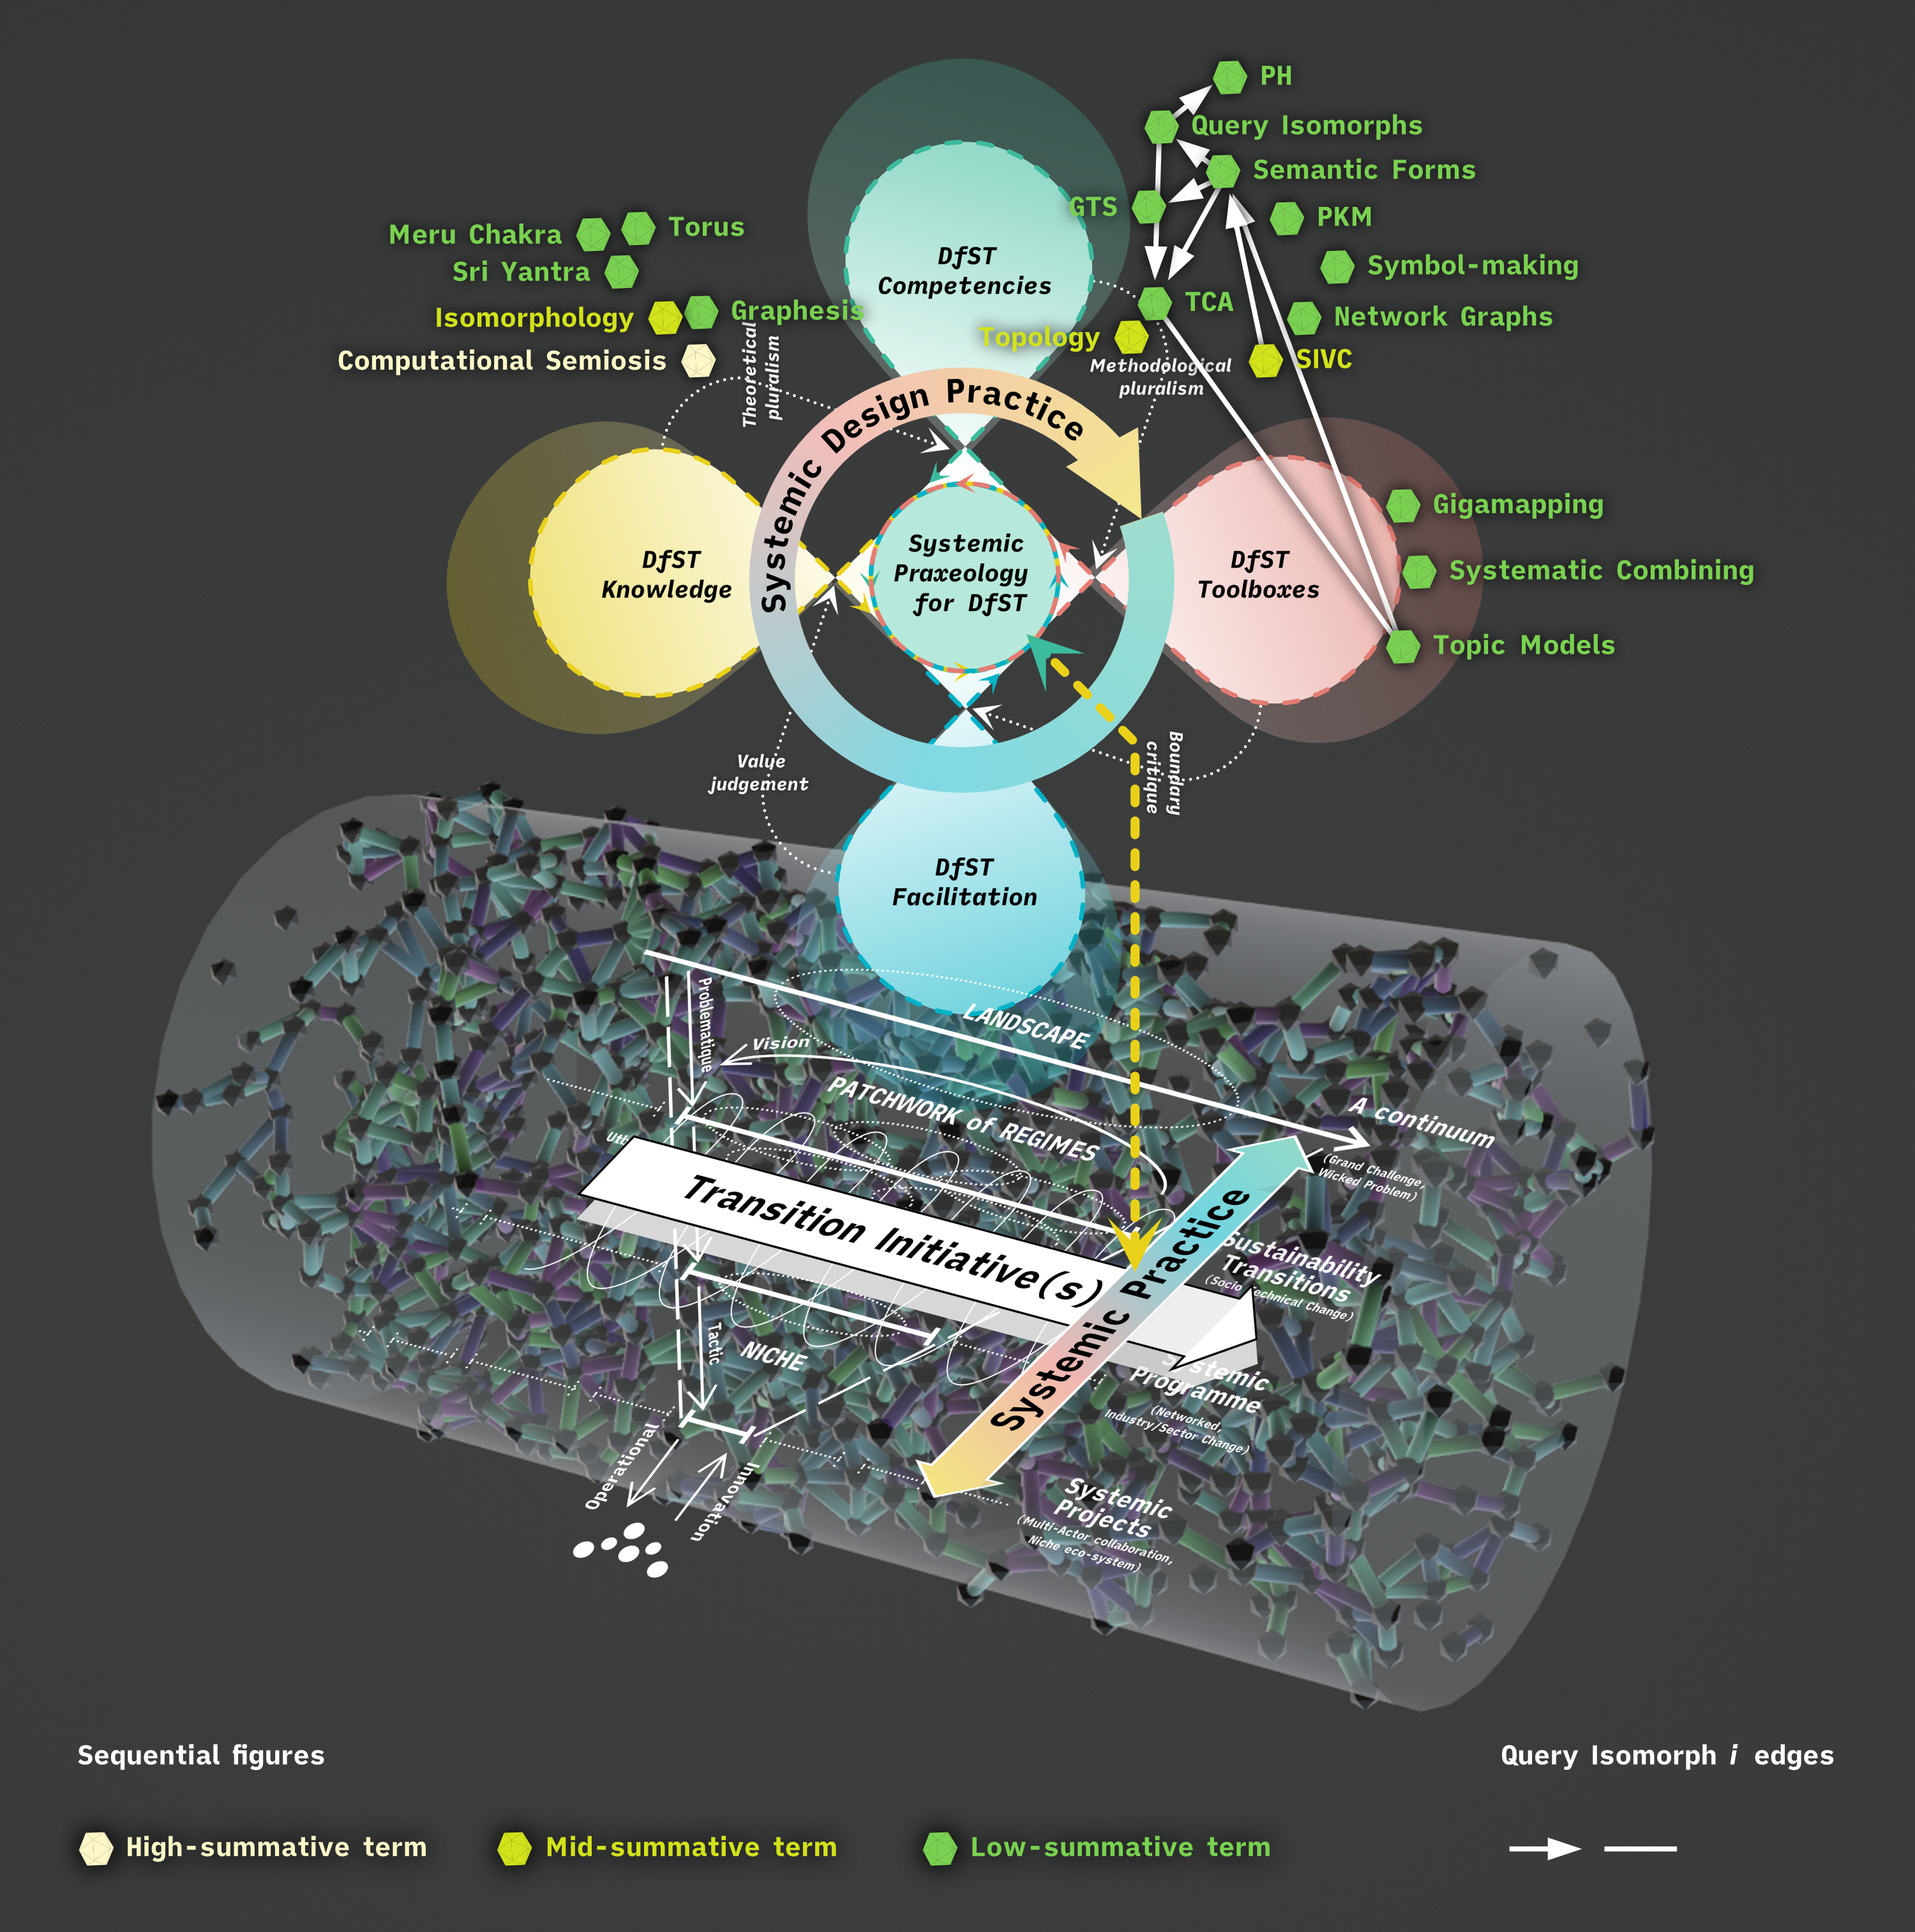
\includegraphics[width=\textwidth]{figures/5.28.Kjode b.png}
    \caption
        [Kjøde's DfST Systematic Combining gigamap visualized as Cylinder Semantic Form network graph with Query Isomorph \textit{i} and Sample \textit{s}]
        {\textbf{
            Kjøde's DfST Systematic Combining gigamap visualized as Cylinder Semantic Form network graph with Query Isomorph \textit{i} and Sample \textit{s}.} The portion of this figure which is \autoref{f5.27} is based on Kjøde’s ``Praxeological framework for DfST relating to systematic transition initiatives” \citep[p. 144]{kjode_entanglement_2024}. Sample \textit{s} terms included for context.
}
    \label{f5.28.Kjode b}
\end{figure}
\FloatBarrier  
\index[people]{Kjøde, Svein Gunnar}
\index[terms]{gigamapping}
\index[terms]{Systematic Combining (SC)}
\index[terms]{Query Isomorphs}





\FloatBarrier  
\subsubsection{LLM as Sphere Semantic Form}
\begin{figure}[h!]
    \centering
    \includegraphics[width=\textwidth]{figures/5.15.Sphere LLM.png}
    \caption[Sphere Semantic Form as LLM Vector Embeddings]
    {\textbf{Sphere Semantic Form as LLM Vector Embeddings.}
}
    \label{f5.15.Sphere LLM}
\end{figure}
\FloatBarrier  

Although LLMs can rely on graphs of text, such as vector embeddings, they are not intended as information visualization. For a model to be usable as AI, it seems to requires a high-dimensionality that embed thousands of dimensions. In this sense LLM vector graphs are beyond visuospatial representation. They cannot be seen or captured spatially, at least not without compromising the semantic value of its dimensional interrelationships by using dimensionality reduction.

I turn here to Grant Sanderon’s illustrations of vector space, which show how LLMs organize ideas as radii around a central origin point \citep{sanderson_attention_2024}. Vector embeddings operate as the direction of a line- or vector- in space, but individual node positions work differently. However, the specificity of a vector still allows for graphing individual coordinates, though variable, with the use of topology, which is less concerned with exact coordinates. Query Isomorphs may be compatible with the LM vector graph; for the sake of UI, Query Isomorphs may be input as individual points but searched along vector lines within an LM. In this way, the LM is an example of a Sphere Semantic Form and a prospect for using Query Isomorphs within texts or groups of texts. This treatment of LM vector graphs opens up interoperability with network graphs, and their spherical composition can be represented and leveraged as a Semantic Form.
\index[terms]{Language Model (LM)}
\index[terms]{Large Language Model (LLM)}
\index[terms]{topology}
\index[terms]{Query Isomorphs}



\subsubsection{Section conclusion}

I propose that by using Systematic Combining and other forms of Systemic Design in the Design for Sustainability Transitions (DfST), Kjøde and I are engaging in a Systemic Design for Sustainability Transitions (SDfST). However, building on Pangaro, TCA Workspace is a ``Conversation to Design the Designing" \citep[p. 185]{pangaro_design_2011}. By proposing the design of a computational expansion of SDfST and using meta-Systematic Combining, my work is, then, a meta-design of SDfST.
\index[terms]{Systemic Design} \index[terms]{Design for Sustainability Transitions} 
\index[people]{Pangaro, Paul} \index[terms]{TCA Workspace} \index[terms]{Systematic Combining (SC)}
\index[people]{Kjøde, Svein Gunnar}

As a member of the Systemic Design Association (SDA), I have witnessed the rising popularity of Systems Oriented Design and Systemic Design with the use of gigamaps \citep{sevaldson_giga-mapping_2011,sevaldson_designing_2022}. As a student at OCAD University’s Digital Futures program, I have witnessed the increased use of virtual three-dimensional visualization in game design, interface design, and LMs. Spaces with a codified practice like Systems Oriented Design and Systemic Design would benefit from a self-awareness of composition forms to diversity their practitioner base. Furthermore, practitioners of three-dimensional visualizations and Systemic Design Practitioners both are poised to benefit from applying LM-assisted mathematical approaches to graph analysis like TDA and TCA if they were to use a tool like TCA Workspace.
\index[terms]{Topological Data Analysis (TDA)}
\index[terms]{Topological Capta Analysis (TCA)}
\index[people]{Sevaldson, Birger}
\index[terms]{Systems Oriented Design (SOD)}

Semantic Forms, Query Isomorphs, and TCA Workspace represent how my work is a visuospatialization of theory. Semantic Forms emerged from my survey of symbols, Query Isomorphs are a means of examining isomorphologies within the Semantic Form isomorphs, and TCA Workspace is a means to incorporate both Semantic Forms and Query Isomorphs within the larger practice of codifying three-dimensional modes of Visuospatial Knowledge Activation.
\index[terms]{Knowledge Activation (KA)} 
\index[terms]{Semantic Forms} 
\index[terms]{Query Isomorphs} 
\index[terms]{Visuospatial Knowledge Activation (VKA)} 
\index[terms]{TCA Workspace}
\index[terms]{visuospatialization}
\index[terms]{visuospatial epistemology}
\clearpage






\section{From visuospatial models to theory and method}
The following contributions are ways my visuospatial models inform my theoretical and methodological proposals that build on my literature review: C3. Ontological Semantic Network Summary (OSNS), C4. Symbol-setting, C5. Terroir of Text and Graphs (TTG), and C6. TCA Researcher Grouping. 
\index[terms]{Ontological Semantic Network Summaries (OSNS)}

\subsection{Contribution 3. Ontological Semantic Network Summaries}
\begin{enumerate}
     \item[\textbf{C3}] \textit{Ontological Semantic Network Summaries (OSNS)} as a means of revealing ontological relationships between ideas in a given body of research using HITL CATG, HATG, or both.

\end{enumerate}

Considering the significance of the Tree of Porphyry, I propose Ontological Semantic Network Summary (OSNS) as a framework for human-in-the-loop semantic network mapping of ontologies in an LM or group of texts. Developing such summaries would assist researchers in identifying the inheritance of key ideas in the logic of a text or body of texts as a tool for its own sake, and to categorize sources in reference pools.
\index[terms]{Large Language Model (LLM)}
\index[terms]{Language Model (LM)}
\index[terms]{Tree of Porphyry}
\index[terms]{Ontological Semantic Network Summaries (OSNS)}

The operationalization of OSNS would accelerate choosing from among research resources, including the choice between groups of texts and Language Model aggregates of texts. The graphic simplicity of the Tree of Porphyry offers an entry point for more complex representations that integrate the insights of this study. For instance: dimensional addition into a three-dimensional OSNS would accommodate more nodes; quantification of nodes and vectors would indicate more or less influence of a particular idea; the analysis of degree-difference can be used among network graph vertices; Query Isomorphs using Topological Capta Analysis and small graph chunks can be used to derive more information from OSNS; Semantic Form configuration can be used to reveal semantic compositions in OSNS; TTG can be used to to examine text and its OSNS in relationship to place; Symbol-setting can articulate culturally-specific summaries of insights in conjunction with OSNS; last, OSNS can be used to reveal alignment between researchers in universities and among other research organizations.
\index[terms]{Terroir of Text and Graphs (TTG)}
\index[terms]{Symbol-setting}
\index[terms]{Tree of Porphyry}
\index[terms]{Topological Capta Analysis (TCA)}
\index[terms]{Ontological Semantic Network Summaries (OSNS)}

\autoref{f6.1} is an example of what a simple two-dimensional Ontological Semantic Network Summary of the \textit{Great Works of the Western World} (1952) would look like by overlaying the terms of the \textit{Syntopicon} \citep[p. xii]{adler_great_1952-2} onto the Tree of Porphyry \citep[p. 4-5]{sowa_knowledge_2000}. This example is simplified by the shared Aristotelian orientation of Adler, Sowa, and Porphyry, but a fully realized computationally-produced OSNS would produce graphs for texts from more diverse semantic fields.


\index[people]{Sowa, John F.}
\index[people]{Adler, Mortimer J.}
\FloatBarrier  
\begin{figure}[h]
    \centering
    \includegraphics[width=\textwidth]{figures/6.1.png}
    \caption[An Ontological Summary Graph of the Syntopicon’s Great Ideas onto the Tree of Porphyry]
    {\textbf{An Ontological Summary Graph of the Syntopicon’s Great Ideas \citep[p. xii]{adler_great_1952-2} onto the Tree of Porphyry \citep[p. 4-5]{sowa_knowledge_2000}.}}
    \label{f6.1}
\end{figure}
\index[terms]{Syntopicon}
\index[terms]{Tree of Porphyry}
\index[terms]{Ontological Semantic Network Summaries (OSNS)}
\FloatBarrier  
\clearpage

\subsection{Contribution 4. Symbol-setting}
\begin{enumerate}
        \item[\textbf{C4}] \textit{Symbol-setting}, a method for expanding the semiotic range of knowledge production using symbol co-creation in HITL CATG, HATG, or both.
\end{enumerate}
\index[terms]{Symbol-setting}
The relationship between word and symbol is fluid and dynamic, so a treatment of approaches that use symbols in KA follows. Symbol-setting is my proposed framework to expand word-based definition to include visuospatial modalities of symbolic co-production. 
\index[terms]{Symbol-setting}

Carl G. Liungman (or in other texts Ljungman) categorized the composition of a wide array of symbols from a variety of cultural contexts and academic disciplines in \textit{Thought Signs} (1995)\footnote{Liungman categories are more intricate, but they generally group symbols by symmetry, openness, straightness of line, and the crossing of lines \citep[p. 49-93]{liungman_thought_1995}.}. While Liungman includes symbols from outside of Europe, and similarly to Adler’s work, Liungman's collection of symbols center Western intellectual tradition. I do not propose Liungman’s work as a universal categorization but as a starting point for the practice of categorizing the composition of symbols that inform their collaborative co-production. 
\index[people]{Adler, Mortimer J.}
\index[people]{Liungman, Carl G.}

Symbol-setting can benefit from various practices to represent a community’s perspective. Branding, which might come to mind to the reader first in a design context, lends itself to a variety of tools and research approaches for the production of symbols. For example, symbol-setting already happens to a degree in making pictographs, UX icons, and emojis. Gigamapping \citep{sevaldson_giga-mapping_2011} and Systematic Combining \citep{kjode_entanglement_2024} are already a kind of symbolic co-production through the use of graphs, and are thus a form of Symbol-setting. Additionally, they lend themselves to Symbol-setting by co-creating Liungman thought signs that integrate an idea or a combination of ideas into a glyph. Symbol-setting can even be hierophanic, as discussed in my earlier comments on Eliade, and a part of a community’s understanding of the manifestation of the divine or transcendent \citep[p. 11]{eliade_sacred_1987}. Symbol-setting, in short, is a visuospatial form of knowledge production that can impact a broad range of experiences. 
\index[people]{Sevaldson, Birger}
\index[people]{Kjøde, Svein Gunnar}
\index[terms]{Systematic Combining (SC)}
\index[people]{Liungman, Carl G.}
\index[terms]{gigamapping}
\index[terms]{Symbol-setting}
\index[people]{Eliade, Mircea}


I believe the visuospatial co-production of the symbol is underdeveloped in the design space, systemic and otherwise. Pangaro’s conversational model of co-evolutionary design for narrowing and expanding language \citep[p. 185]{pangaro_design_2011} and Equity-Centered Community Design (ECCD) “language setting” \citep[p. 8-11]{creative_reaction_lab_equity-centered_2018} can both benefit from Symbol-setting. By providing new ways to arrive at a common understanding, TCA Workspace would facilitate conversations across academic and power differences by empowering equity-oriented approaches like ECCD.  
\index[terms]{TCA Workspace}
\index[people]{Pangaro, Paul}
\index[people]{Carroll, Antionette D.}

By proposing Symbol-setting, I aim to support co-creative KA that uses more interpretative facets of visuospatial epistemology in producing “thought signs” \citep{liungman_thought_1995}. When practiced in TCA Workspace, Symbol-setting would take the forms and hyper-forms of multidimensional text analysis and expand the capabilities of various design practices.
\index[terms]{TCA Workspace}
\index[people]{Liungman, Carl G.}
\index[terms]{visuospatial epistemology}
\index[terms]{Symbol-setting}
\clearpage

\FloatBarrier  
\subsection{Contribution 5. Terroir of Text and Graphs}
\begin{enumerate}
        \item[\textbf{C5}] \textit{Terroir of Text and Graphs (TTG)}, a method of HITL CATG that uses TCA to interpret and reveal semantic relationships between (a) texts and graphs, and (b) the features and systems of ecological place.
\end{enumerate}
\index[terms]{Terroir of Text and Graphs (TTG)}
\begin{figure}[h]
    \centering
    \includegraphics[width=\linewidth]{figures/6.2.png}
    \caption[Torus vs Silos]
    {\textbf{Torus vs Silos.} Illustration of spatial gigamap with Horn Torus Semantic Form text network graph. This example visualizes an analysis of three siloed hyper-specialized work ``communities" and three agricultural monoculture operations nearest them in the same province or municipality. This model proposes TCA to identify solutions for siloed over-work \textit{and} extractive monoculture agriculture.}
    \label{f6.2}
\end{figure}
\index[terms]{Horn Torus Semantic Form}
\index[terms]{gigamapping}
\FloatBarrier

I first learned about wine from my father, who taught my brother and me to taste for region. It is from viticulture that I borrow the term \textit{terroir}, where the term is used to relate ``the sensory attributes of wine to the environmental conditions in which the grapes are grown”, which involves considering interacting factors like ``climate, soil, cultivar, and human practices” \citep[p. 1]{van_leeuwen_concept_2006-1}. In \textit{The Caribou Taste Different Now}, editors Gérin-Lajoie et al. present observations by Inuit elders of how climate change is causing such drastic changes to flora and fauna that it can be perceived by taste \citep[p. 35, 71, 72, 86, 269, 280, 281] {gerin-lajoie_caribou_2016}. The embodied urgency of a human need for food serves as a reminder to me about how connected and vulnerable we all are to climate change. The trans-sensorial synaesthetic quality of tasting information about global warming is the \textit{terroir} in Terroir of Text and Graphs (TTG), which is itself a trans-modal Topological Capta Analysis of the land-thought relationship.
\index[terms]{Terroir of Text and Graphs (TTG)}
\index[terms]{Indigeneity}


The relationship between place and language influences fundamental characteristics of how we think. As an example of how this plays out in the materiality of language the rounded wavy lines that characterize many scripts from Southern India are “usually explained as a result of the exigencies of writing with a stylus on palm leaves” \citep[p. 39]{salomon_indian_1998}. Of course, many other types of relationships exist between place and language. So, I propose TCA as a method for examining relationships between the ecological and conceptual to improve the translation of information from one ecologically located way of knowing to another. I anticipate that by using interdisciplinary ecological TCA we will observe more numerous and complex forms of the Terroir of Text and Graphs.
\index[people]{Tversky, Barbara}

%To apply Tversky’s research on the neuroscience of the visuospatial \citep{tversky_barbara_2022}, one might examine differences in metaphor to the verticality and horizontality of place; one would expect the semantic value of verticality would differ considerably between communities living in perilous high altitude when compared to communities living near sea-level. 

Examining the relationship between place and idea using TCA in TTG has significant implications for understanding contemporary classifications of city, country, and wilderness. In \autoref{f6.2}, my illustration of a spatial gigamap with a Horn Torus Semantic Form network graph, I propose that rewilding as a means of ecological diversity in food supply can consiliently inform the diversification of interdisciplinary forums in academic settings. Such a model would derive insight from solutions in sustainable climate-resilient polyculture food production methods as a means of assuaging the ecological risks of overreliance on agricultural monoculture \citep[p. 1]{altieri_agroecology_2015}. Applying said solutions to siloed hyper-specialized monocultural over-work could provide insight into the best types of opportunities for disciplinary inter-pollination solutions. These and other entry points to relief via systemic analysis can be expected from developing Topological Capta Analysis into a wider de-siloing practice like TTG where text and graphs are examined in relation to frameworks outside their discipline and location of origin using HITL CATG.
\index[terms]{Horn Torus Semantic Form}
\index[terms]{gigamapping}
\index[terms]{rewilding}
\index[terms]{Terroir of Text and Graphs (TTG)}

Developing a TCA practice to understand TTG would go on to address gaps that were not covered in this study, namely empirical and spatial gaps. Empirically, we could collect data or create capta to fully understand text terroir through data model experiments. Spatially, understanding the relationship between text and place is limited compared to what can be achieved with a text terroir analysis. Expanding research on Query Isomorphs using TCA and TTG could provide new insight into interregional relationships to empower underrepresented areas. As I will discuss later, TTG can bolster new climate justice and resilience technologies if adjoined to Indigenous approaches to Artificial Intelligence.
\index[terms]{Indigeneity}
\index[terms]{Terroir of Text and Graphs (TTG)}
\index[terms]{capta}
\index[terms]{climate justice}

My TTG model \textit{Torus vs Silos} illustrates the way Topological Capta Analysis could map relationships between ecological and informational using Semantic Forms, Query Isomorphs and visuospatial gigamapping. \autoref{f6.2} visualizes an analysis of three siloed hyper-specialized and overworked groups of people and three extractive agricultural monoculture operations nearest them. Using TTG in this way, I would seek to reveal parallels of extractive capitalism that are at play in both ecological space and idea space to support their transition into more anthropo-symbiotic\footnote{The term \textit{anthropo-symbiotic} is borrowed from Fonseca et al.'s \textit{Anthropo-symbiotic ethics: a path to the sustainability of life} which discusses ethical ``theories with a more conciliatory and balanced view about the relation between the environment, humans and animals" \citep{fonseca_anthropo-symbiotic_2022}.} ways of being and knowing. 
\index[terms]{Indigeneity}
\index[terms]{Terroir of Text and Graphs (TTG)}
\index[terms]{Query Isomorphs}
\index[terms]{Topological Capta Analysis (TCA)}
\index[terms]{Artificial Intelligence (AI)}

TTG would more explicitly delineate relationships between land and language in human and non-human ways of knowing. From an Indigenous perspective, the wisdom carried in story and cultural practice can be articulated through the expanded field of graphs of texts, including Semantic Forms, Query Isomorphs and TCA Workspace in gigamaps, Systematic Combinations, topic models, and the vector graphs that form the basis of AI Large Language Models. TTG as the integration of diverse wisdom lineages, including the distinctly anthropo-symbiotic Indigenous ways of knowing, can be simultaneously an act of ecojustice and a means of informing Sustainability Transitions. At the core of TTG is my commitment to Indigenous data sovereignty \citep[p. 12]{lewis_abundant_2024} in which ``Indigenous practitioners are making the decisions that guide the development of AI themselves" \citep[p. 8]{lewis_abundant_2024}. A TTG-based HITL CATG of fields like ethnobotany, ethnoecology\footnote{Turner et al. define the interrelated fields of ethnobotany and ethnoecology \citep[p. 6-8]{turner_introduction_2020}.}, biocultural memory 
\footnote{Monterrubio-Solis et al. define biocultural memory as follows: ``Biocultural memory refers to the human reliance on intergenerational relationships, not only to one another but within territories, where the physicality of agroecosystems, material and symbolic meanings, as well as institutions join to constitute biocultural memory” \citep[p. 2]{monterrubio-solis_narrating_2023}.}, plant-human co-evolution is part of my plan for TCA Workspace Knowledge Activation.
\index[terms]{Terroir of Text and Graphs (TTG)}
\index[terms]{TCA Workspace}
\index[terms]{Systematic Combining (SC)}
\index[terms]{gigamapping}
\index[terms]{Indigeneity}

\subsubsection{Land and Indigeneity}
On a personal level, this thesis research has been driven by my work to honour and reconnect with my South American Indigenous roots which were kept from me by ruling powers, buried by colonialism and xenophobia. In my research about the development of computational tools that support climate justice and resilience alongside Indigenous perspectives, I seek collaborators who share these goals. 
\index[terms]{Indigeneity}

I have found alignment with the Abundant Intelligences project, an international research effort spanning Canada, the United States, and New Zealand. Jason Edward Lewis, professor of computation arts at Concordia University and the University Research Chair in Computational Media and the Indigenous Future Imaginary, is co-leading the Abundant Intelligences project. Lewis et al. assert that the way AI is developed at present is limited by ``Western rationalist epistemologies that exclude many ways of knowing", so, ``the systematic operationalization of bias against non-white, non-male, and non-Western peoples" is also unable to ``adequately, robustly, and humanely conceptualize intelligence-much less attempt to replicate it" \citep[p. 1-2]{lewis_abundant_2024}.
\index[terms]{Indigeneity}


``To govern ourselves means to govern our stories and our ways of telling stories" \citep[p. 19]{maskegon-iskwew_drumbeats_2005}\footnote{Maskêgon-Iskwêw cites this text from the general ``principles for the development of Indigenous networked art production" formalized during the \textit{drumbeats to drumbytes} gathering at The Banff Centre in March 1994 \citep[p. 19]{maskegon-iskwew_drumbeats_2005}.}. If unchecked, AI will continue to exacerbate oppression and marginalization by expanding the tools of imperialism and colonization. The stakes of critical AI research like the Abundant Intelligences project are high and growing higher. 


The OCAD University pod for Abundant Intelligences is called the \textit{A Dish with One Spoon––Towards ``Generous AI” Invention and Collaboration} project and led by co-investigators Dr. Sara Diamond and Archer Pechawis. Our emerging team will draw upon Indigenous frameworks to offer redefinitions of intelligence and develop computational practices that refashion AI from being tools of ``exclusion, extraction, and eradication into engines for increasing our care of one another and our world" \citep{visual_analytics_lab_abundant_2024}. I am honoured to be given the role of the first OCAD U Research Assistant for Abundant Intelligences, working closely with Peter Morin, Ruth Green, and Susan Blight.


Pechawis and Diamond both worked closely with the late Âhasiw Maskêgon-Iskwêw (1958-2006), Cree/French Métis performance artist, theorist, and creator of \textit{isi-pîkiskwêwin-ayapihkêsîsak (Speaking the Language of Spiders)} \citep{maskegon-iskwew_isi-pikiskwewin-ayapihkesisak_1996}. Maskêgon-Iskwêw's work is so often extolled and remembered in our meetings that he frequently feels like a third mentor on the beginnings of my journey through Indigenous Artificial Intelligence. I muse about asking him about the animate web in hyperspace, decentralization of ideas' provenances by reason-automatons, opportunities of using rhi-zombies to transubstantiate the poisons of ecocide, mitigating the risks of becoming its host/s in a tangle of disinformation and illusion.
\index[terms]{rhizome}
\index[terms]{rhi-zombie}
\index[terms]{Indigeneity}
\index[people]{Maskêgon-Iskwêw, Âhasiw} 
\index[terms]{A Dish with One Spoon}


I am cautiously optimistic about using Large Language Models in Two-Eyed\footnote{Two-Eyed Seeing as a principle was ``advanced by Canadian Indigenous leaders, notably Mi'kmaw Elders Albert and Murdena Marshall" \citep[p. 3]{bourgeois-doyle_two-eyed_2019}.} AI frameworks that draw strengths from both Indigenous and Western ways of knowing \citep[p. 3]{bourgeois-doyle_two-eyed_2019}. To echo Bourgeois-Doyle, I am committed to a critical evaluation of TTG to maintain a Two-Eyed Seeing model for Topological Capta Analysis, with and without AI, which works for ``integrated thinking, respectful multidisciplinary collaboration, and transcending combinations of interests for public good" \citep[p. 3]{bourgeois-doyle_two-eyed_2019}. To echo Leroy Little Bear, this good must not be limited to humans, but must also include the welfare of the entire spider web of our relations \citep[p. 78, p. 84]{little_bear_jagged_2000}.
\index[terms]{Indigeneity}
\index[terms]{Terroir of Text and Graphs (TTG)}
\index[people]{Little Bear, Leroy}





\clearpage

\subsection{Contribution 6. TCA Researcher Grouping}
\begin{enumerate}
        \item[\textbf{C6}] \textit{TCA Researcher Grouping}, a proposal to use TCA for grouping research collaborators more effectively using HITL CATG, HATG, or both.
\end{enumerate}
Developing Computational Analysis of Texts and Graphs (CATG) can improve our work relationships in research institutions. As the administrative arm of TCA Workspace, TCA Researcher Grouping could manage rich graph databases to group researchers more effectively, benefiting expansion of research projects and connecting with new talent.
\index[terms]{TCA Researcher Grouping}


As a means of operationalizing CATG, TCA Workspace and TCA Researcher Grouping have the potential to catalyze solutions with more effective cross-pollination of disciplines. When applied to ecological climate resilience efforts, TCA Workspace could become a symbiotic permaculture of knowledgeways and Earth custodianship, rewilding in and beneath the computer.

\index[terms]{TCA Workspace}
\index[terms]{rewilding}
\index[terms]{TCA Researcher Grouping}
\index[terms]{climate resilience}